% Copyright 1994 Peter Williams.
%
% This work may be distributed and/or modified under the
% conditions of the LaTeX Project Public License, either version 1.3
% of this license or (at your option) any later version.
% The latest version of this license is in
%   http://www.latex-project.org/lppl.txt
% and version 1.3 or later is part of all distributions of LaTeX
% version 2005/12/01 or later.
%
% This work has the LPPL maintenance status `maintained'.
% 
% The Current Maintainers of this work are Peter Williams and Thorsten Schnier.
%
% This work consists of all files listed in manifest.txt.
%
% Licence and copyright notice added on behalf of Peter Williams and Thorsten Schnier
% by Clea F. Rees 2009/01/30.
% \begin{filecontents}{bibtexlogo.sty}
% \def\lowBibTeX{{\reset@font\rmfamily B\kern-.05em%
%  \raise.0ex\hbox{\scshape i\kern-.025em b}\kern-.08em%
%  T\kern-.1667em\lower.7ex\hbox{E}\kern-.125emX}}


%\def\BibTeX{\protect\lowBibTeX}
%\end{filecontents}
\documentclass[a4paper]{article}
\usepackage{harvard}
\usepackage{bibtexlogo}
\usepackage[swedish]{babel} % Svenska
\selectlanguage{swedish} % Välj språk
\usepackage[T1]{fontenc}
\usepackage[utf8]{inputenc}
\usepackage{graphicx}
%\usepackage{fullpage}
\usepackage{titlesec}
\newcommand{\sectionbreak}{\clearpage}
\usepackage{caption}
\usepackage[a4paper]{geometry}
\usepackage{setspace}
\usepackage{listings}
%\usepackage{float}
%\restylefloat{table}
\usepackage{tikz}


\renewcommand{\baselinestretch}{1.5}



\newcommand{\comname}[1]{{\bf $\backslash$#1}}
\newcommand{\keyword}[1]{{\bf #1}}
\newcommand{\varname}[1]{{\em #1}}
\newcommand{\harvard}{{\sf harvard}}
\newcommand{\Harvard}{{\sf Harvard}}

\pagenumbering{roman}

\title{Titelsida}
\author{David Anderson \and Simon robertsson}

\hyphenation{cite-as-noun poss-ess-ive-cite cit-at-ion-mode cite-year
cite-name bib-lio-gr-aphy-sty-le cit-at-ion-sty-le har-vard-par-en-this
har-vard-year-par-en-this har-vard-item bib-item har-vard-and use-pack-age}

\begin{document}




\bibliographystyle{agsm}
\maketitle


\begin{tikzpicture}[remember picture,overlay]
\node[inner sep=0pt] at (current page.center) {
\includegraphics[page=1]{front}};
\end{tikzpicture}
\clearpage

\newpage

\begin{abstract}
De senaste decennierna har stora reformer genomförts inom den svenska offentliga sektorn. Dessa reformer har förändrat sättet vårdorganisationer styrs. Ett koncept som idag implementeras på flera institutioner är Värdebaserad vård (VBV). Grundtanken bakom VBV är att maximera värdet som produceras genom att maximera kvaliteten i förhållande till kostnaden.

Syftet med detta arbete är att undersöka hur värdeskapande mäts inom VBV genom att jämföra värdeskapande mellan två vårdenheter på Karolinska sjukhuset i Solna och Huddinge. Resultatet av jämförelsen visar att det finns små skillnader i värdeskapandet. Det framgår även att det inte råder någon konsensus om hur värde ska mätas, vidare forskning efterfrågas följaktligen inom detta område.
\end{abstract}

\tableofcontents

\newpage

\listoffigures
\begingroup
\let\clearpage\relax
\listoftables
\endgroup

\newpage

\clearpage
\pagenumbering{arabic} 

\section{Inledning}

Under de senaste decennierna har stora reformer genomförts inom den svenska
offentliga sektorn. Många av de förändringar som genomförts är baserade på
styrformer från den privata sektorn och innefattar ökad konkurrensutsättning och
starkare resultatfokus. Inom vård och omsorg är det tydligt hur dessa reformer
ändrat det sätt vårdorganisationer styrs. Det är numera inte bara lagar,
politiska beslut och skattefinansiering som ligger till grund för
organisationsstyrning inom den offentliga sektorn. Även marknadsorienterade
inslag såsom konkurrens mellan vårdgivare, resultatfokus samt ekonomisk
resultatstyrning är nu centrala delar. Dessa förändringar har fått konsekvenser
både för personalen inom organisationerna samt för vårdtagre. Ett begrepp som
ofta används för att beskriva det ökade marknadsinslaget inom offentlig sektor är New Public Management (NPM), detta begrepp återkommer senare i detta arbete (Karolinska Institutets folkhälsoakademi, 2011).
 
Den ökade konkurrens vårdgivare ställts inför genom införandet av NPM har lett till att många vårdorganisationer implementerat koncept från näringslivet för att maximera sin kvalitet. Ett sådant koncept är Lean produktion\footnote{ Lean är ett begrepp inom kvalitetsförbättring som bygger på arbete med ständiga förbättringar (Toyota, 2015)}. Ekonomerna Michael Porter och Elizabeth Teisberg har utvecklat ett annat kvalitetförbättringskoncept som kallas värdebaserad vård (VBV). VBV har fått genomslag inom den svenska sjukhussektorn och det centrala ligger i att sätta patienten i fokus. Syftet med VBV är att skapa värde för patienten - värde mätt i patientens hälsa och upplevelser av vården. Detta uppnås genom att leverera högsta möjliga kvalitet för patienten i förhållande till kostnaden för vården (Porter \& Tiesberg, 2006).
 
Ett sjukhus som i dagsläget arbetar med att implementera VBV är Karolinska universitetssjukhuset (Karolinska). Karolinska har årligen 1,5 miljoner patientbesök och är en av Sveriges största vårdgivare (Karolinska, 2015). Målet med införandet av VBV är att uppnå ökad kvalitet utan att öka vårdkostnaden (Wiklund, 2015).

\subsection{Problemdiskussion}

Införandet av NPM och dess styrformer inom den svenska sjukvården har mött mycket kritik. Flera läkare har protesterat mot den ökade byråkratin och att de i dagsläget känner sig mer som företagsledare än vårdgivare (SVT, 2014). Artikelserien “Den olönsamma patienten”, som publicerades i DN under 2013, författad av Maciej Zaremba riktar stark kritik mot NPM. Zaremba menar att dessa reformer lett till att fokus flyttats från patienten och istället styrs organisationerna mot ekonomiska resultat.
 
VBV-konceptet lägger fokus på att skapa så hög kvalitet för patienten som möjligt i förhållande till vårdkostnaden. Därför ser en del VBV som en lösning till flera av de problem NPM skapat eftersom utgångspunkten i konceptet är patientens upplevelse av vården och inte det ekonomiska resultatet (Nordenström, 2014). Kritiker menar dock att VBV bara är en förklädd variant av NPM och att VBV egentligen lider av samma brister. Ingemar Engström, ordförande för Svenska Läkarsällskapets delegation för medicinsk etik, menar att det inte är möjligt att implementera VBV då det är svårt att mäta värdeskapandet i praktiken. Inte minst eftersom många andra faktorer än sjukvårdens kvalitet också påverkar utfallet hos patienten, till exempel socioekonomiska förhållanden och patientens livsstil (Läkartidningen, 2014;111:CPE9).
 
Karolinska är intresserade av att jämföra sina två hjärtinfarktsenheter i Huddinge respektive Solna ur ett värdeskapande perspektiv som en del av implementeringen av VBV-konceptet. Karolinska vill jämföra skillnaden då Solna rankats dåligt i jämförelse med Huddinge i riksgenomsnittet för “Andel döda inom 28 dagar efter sjukhusvårdad hjärtinfarkt” medan Huddinge har lägre dödlighet än riksgenomsnittet (Social- styrelsen, 2013). En möjlig orsak till Solnas förhållandevis dåliga ranking är att deras patientpopulation består av mer svårbehandlade patienter jämfört med genomsnittet. (Wiklund, 2015) Den snedvridande jämförelseeffekten av patientpopulationer är ett uppmärksammat problem inom VBV. För att komma tillrätta med problemet så kan metoder som, justerar för eventuella skillnader populationer emellan användas. (Nor- denström, 2014, s. 60).

Värdeskapande är inget nytt koncept, 1985 lanserade Porter konceptet värdekedjan som används inom traditionell verksamhetsstyrning. Här avses en processmodell där värdeskapande aktiviteter identifieras och utvecklas i syfte att maximera vinst och minimera kostnader (Porter 2008). Detta arbete avser begreppet värdeskapande som det används inom VBV, ett koncept som lanserades av Porter \& Tiesberg (2006). Grundtanken är liknande men istället för att maximera vinst eftersträvas här att maximera den patientupplevda kvaliteten inom vårdprocessen. Är det möjligt att applicera värdebegreppet inom vården? och vad krävs för en lyckad implementering? Dessa är exempel på frågor som behandlas i detta arbete.

\subsubsection{Syfte och frågeställningar}

Syftet med detta arbete är att undersöka hur värdeskapande mäts inom vården genom att jämföra värdeskapandet mellan två vårdenheter på Karlonska.

Mer specifikt avser arbetet att besvara följande frågeställningar:

\begin{itemize}
  \item Hur mäts och jämförs värdeskapande inom VBV?
  \item Vilka svårigheter finns vid utformningen av mätningen?
  \item Vad krävs för att en implementering av VBV skall uppnå önskat resultat?
\end{itemize}

\section{Teori}

De teorier som presenteras i detta kapitel fungerar som bakgrund till, de i detta arbetet centrala begreppen NPM och VBV. Dessutom presenteras ett ramverk vilket används för att genomföra den jämförande analysen av vårdenheterna.

\subsection{New public management}

NPM är en uppsättning idéer som under de senaste 30 åren kraftigt präglat tankarna kring hur den offentliga förvaltningen bör utformas (Roland Almqvist 2006, s. 10). NPM:s ursprung och godkännande är omstridd. En tolkning av NPM:s framväxt är att NPM växte fram ut idéströmmarna ‘New Institutional Economics’ och ‘Managerialism’. ‘New Institutional Economics’ bygger på idéer om den öppna marknaden, valfrihet, transparans och incitamentstrukturer som blev populära efter andra världskriget. ‘Managerialism’ innebär i princip att managementmetoder från den privata sektorn appliceras inom den offentliga sektorn. Även om ‘New Institutional Economics’ och ‘Managerialism’ utgör den intellektuella grunden för NPM så har dess framväxt inte skett i vakuum. Hood (1990) påstår i sin tongivande artikel “A New Public Management for all seasons” att det går att urskönja fyra stora trender som ligger till grund för NPM:s framväxt under det sena 1980-talet.

\begin{enumerate}
  \item Ett försök att sakta ned och backa statens tillväxt med avsikt på utgifter och antal anställda.
  \item En övergång mot privatisering eller kvasi-privatisering och därmed bort från kärninstitutioner. Större fokus på subsidiaritet vid tillhandahållandet av tjänster d.v.s. att beslut kring statliga tjänster bör tas närmre de medborgare som nyttjar tjänsten.
  \item En utveckling mot automatisering specifikt inom IT för att producera och distribuera publika tjänster.
  \item Utvecklingen av en mer internationell agenda. Mer fokus på generella problem med offentlig förvaltning, policy, beslut och samarbete mellan nationer. Mindre fokus på lokala traditioner och specialisering utifrån individuella länders traditioner.
\end{enumerate}

NPM är följaktligen ett paraplybegrepp för en generell idéströmning snarare än
en specifik teori för hur offentlig förvaltning bör utformas. Däremot finns det
flera försök till att beskriva NPM och dess kärnbudskap. Lena Agevall (2005),
statsvetare vid Linnéuniversitetet och forskare i ämnet, ger en beskrivning av
NPM där hon delar in begreppet i fem doktriner:

\begin{enumerate}
  \item \textbf{Styrning och kontroll:} Mål och resultatstyrning; strängare
  finansiell kontroll (mer värde för varje krona); kontraktsstyrning;
  prestationsersättningar (till exempel skolpeng); jämförelser/benchmarking samt
  granskningar/utvärderingar.
  \item \textbf{Disaggeregering och konkurrens:} Skapandet av kvasi-marknader, konkurrensutsättning och privatisering.
  \item \textbf{Ledningsroller och delaktighet:} Politikerna ska få mer makt över tjänstemän och förvaltning. Detta ska ske samtidigt som duktiga chefer på lokal nivå ska ges möjligheten att målstyra verksamheten. NPM förespråkar alltså både centralisering och decentralisering.
  \item \textbf{Medborgare, kund och delaktighet:} Medborgaren ska få större makt bl.a. genom sitt inflytande som kund.
  \item \textbf{Nytt språk:} Verksamhetsenheter förvandlas till resultatenheter, chefstjänstemän tituleras direktörer, service och omsorg beskrivs i termer av produktion, medborgaren blir kund etc.
\end{enumerate}

Den del av Agevalls beskrivning som är mest central för detta arbete är Styrning och kontroll. Styrning och kontroll fokuserar på att öka effektiviteten samt uppnå “mer värde för pengarna”. Större vikt läggs på efterkontroll av vad som uppnåtts än hur den dagliga verksamheten sköts. Incitament att förbättra verksamheten skapas genom prestationsersättningar och benchmarking (Almqvist 2006, s. 26-27).
 
Styrning och kontroll ligger även till grund för dissagregering och konkurrens. Både för konkurrens mellan offentliga utförare och för utkontraktering av offentlig verksamhet. Utkontraktering av offentlig verksamhet bygger på upphandlingar och vid dessa upphandlingar är kvalitet en central parameter i själva utformningen av kontraktet. I kontraktet specificeras vilket resultat som förväntas uppnås av utföraren. Beställaren har sedan ansvar för att styra och följa upp så att de avtalade resultaten efterlevs. Detta sätter stor tilltro till att resultatmåtten både är mätbara och jämförbara, något som inte alltid är självklart (Almqvist 2006, s. 58-59).
 
NPM möttes av blandade känslor när dess ideér under 1990-talet började få fäste inom den offentliga sektorn. Förespråkarna såg på NPM som en lösning till alla inneboende problem inom offentlig förvaltning. Motståndarna å andra sidan såg på NPM som slutet på alla de demokratiska framsteg som skett under det senaste seklet (Hood, 1990, s. 4). Målstyrning - att politikerna sätter målen och att den handlingsinriktade förvaltningen försöker uppnå dessa var det inslag av NPM som först fick genomslag i Sverige. Under 1990-talet infördes och testades målstyrning i flertalet statliga myndigheter, kommuner och landsting. Konkurrensutsättning och marknadsanpassning debatterades men det skulle dröja innan dessa blev verklighet (Almqvist 2006, s. 10-11).
 
Att NPM fått ett starkt fäste i Sverige är enligt Hood (1995) förvånansvärt då
Sverige har en stark socialdemokratisk tradition, till skillnad från merparten av de andra länder där NPM fått ett stort genomslag. En förklaring till NPM:s starka fäste i Sverige är enligt Hans Hasselsblad den svenska traditionen av samhällelig ingenjörskonst (Hasselblad et al., 2008, s. 10).
 
NPM infördes i de svenska landstingen i början av 1990-talet via kvalitetsstyrningskonceptet Total Quality Management (TQM) på initiativ av den borgerliga regeringen som styrde under tiden. TQM-projektet skrotades med tiden men lämnade stora spår efter sig. Bland annat det Nationella kvalitetsregistret (Hasselblad et al., 2008, s. 123). För närvarade finns det 81 Nationella kvalitetsregister som utgörs av databaser med individbunden data inom specifika medicinska områden (Nationella kvalitetsregister, 2014). Via rapporter från kvalitetsregistren kan läkare, kliniker, sjukhus och landsting analysera förändringar över tid och jämföra sig med andra som deltar i registerarbetet (Hasselblad et al., 2008, s. 124-125)

De Nationella kvalitetsregistren har beskrivits av Socialstyrelsen som det mest framgångsrika instrumentet för uppföljning och kvalitetsutveckling inom hälso- och sjukvården. I takt med arbetet kring kvalitetsregistren har ett antal frågeställningar om dess framtid uppdagats. Exempel på dessa går att se från teman på Kvalitetsregisterdagarna: 2000 - “Stora skillnader i svensk hälso- och sjukvård och vad vi gör åt dem?”; 2002 - “Livskvalitet, patientupplevelser och olika mått på funktionsvinst och patientupplevd nytta”; 2006 - “Blir det bättre för patienterna med kvalitetsregister?”; 2007 - “Öppna jämförelser av resultat”.

Oavsett hur resultatet av NPM tolkas är det tydligt att det gjort avtryck i styrningen av Svensk sjukvård. Stefan Fölster och Jörgen Nordenström, professorer på KTH respektive Karolinska, tillhör dem som försvarar NPM. De påstår att det vi har i Sverige idag inte är NPM, utan snarare något som liknar godtycklig detaljstyrning. Deras recept lyder(http://www.lakartidningen.se/Klinik-och-vetenskap/Kommentar/2015/05/Vardeskapande-styrning-kan-ateruppratta-lakares-inflytande/):

\begin{quotation}
\textit{För att skapa bättre vård och bättre hälsa behöver ett värdeskapande styrsystem införas, som ökar engagemanget hos vårdpersonalen och som sätter vårdens kvalitet och patienternas behov först.}
\end{quotation}

Mot bakgrund av vad diskuteras på Kvalitetsregisterdagarna och vad förespråkare av NPM påstår är det förståeligt att VBV skapat så pass stors intresse. 

\subsection{Värdebaserad Vård}

Värdebaserad vård (VBV) är ett koncept som från början togs fram av Harvarduniversitetets professor Michael Porter. Konceptet innefattar flera av de doktriner som Agevall (2005) presentar och som beskrivs som centrala delar inom NPM. VBV har fått genomslag i flera länder och i Sverige jobbar bland annat två av landets största sjukhus, Akademiska sjukhuset i Uppsala och Karolinska institutet i Stockholm, med att implementera VBV.
 
Syftet med att styra en vårdorganisation enligt VBV är att maximera värdeskapandet inom organisationen. Inom VBV definieras värde som kvalitet hos vården sett i förhållande till hur mycket omhändertagandet av patienten kostat, se ekvation \ref{eq:varde}. (Porter, 2010).

\begin{equation}
\label{eq:varde}
	V \ddot{a} rde = Kvalitet/Kostnad
\end{equation}

Värde är viktigt då det bör vara det yttersta målet hos vårdorganisationer, eftersom det är värdet som i slutändan är viktigast för patienten och även det förenade intresset hos andra berörda aktörer (Porter \& Teisberg, 2006). En värdeökning gynnar patienter, skattebetalare och leverantörer samtidigt som den ökar den ekonomiska hållbarheten i hela vårdsystemet. Detta kan låta självklart och kanske enkelt men det är ovanligt att vårdorganisationer jobbar värdefokuserat. Det är till och med ovanligt att organisationer överhuvudtaget mäter värdet av det som produceras. Porter ser det som en risk är att vård betraktas som en konstform och inte en vetenskaplig process med ständig förbättringspotential (Porter, 2010).
 
Kvalitet defineras av Porter (2010) som:
\begin{quotation}
\textit{The full set of outcomes, adjusted for individual patient circumstances, constitutes the quality of care for a patient.}
\end{quotation}
Kvalitet är således resultatet av vården hos den individuella patienten med hänsyn till dennes individuella omständigheter.

Införandet av VBV har emellertid mötts av kritik från bland annat läkare. Kritiken riktas främst mot att konceptet är framtaget för den amerikanska marknaden där en annan konkurrenssituation råder och där resursfördelningen är betydligt mer ojämlik. VBV bygger på att det är möjligt att mäta vårdresultat vilket är långt från självklart. Kritiker anser att relationen mellan uppdragsgivare och vårdorganisationer måste bygga på förtroende och tillit, inte på missvisande styrmått. De menar att det största problemet med VBV är själva mätningen. Konceptet kan låta bra i teorin men i praktiken kan det vara svårt att genomföra (Läkartidningen. 2014;111:C77E). 

Frågan är om det går att mäta vårdresultat på ett rättvist och fruktbart sätt?

\subsection{Att mäta värdeskapande}

Då det yttersta målet med VBV är att förbättra kvaliteten i förhållande till vårdkostnaden är en central del i detta arbete just att mäta kvaliteten och kostnaden. Att mäta, rapportera och jämföra kvalitet är ett viktigt steg för att motivera personal och i förlängningen öka värdet av det som produceras. För att möjliggöra detta krävs en öppenhet för kartläggning av utfall och kostnader. Med hjälp av insamlad data kan institutioner kartlägga värdeskapandet över tid och även jämföra sitt egna resultat med andra institutioner. Denna typ av kartläggning gör det också möjligt att informera patienter, vårdgivare och beslutsfattare om det relativa värdet vårdorganisationen skapat. Det absolut viktigaste incitamentet med denna typ av rapportering är dock att skapa ett underlag för att kunna stärka värdeskapandet i organisationen - att öka kvaliteten i förhållande till kostnaden (Nordenström, 2014, s. 59).

\subsubsection{Att mäta kvalitet}

Som tidigare nämnts är en del av värdeskapandet att uppnå så hög kvalitet som möjligt. Det är således viktigt att kunna mäta kvalitetsskapande. Vid utvärdering och granskning av kvalitet inom sjukvården används två huvudsakliga typer utav mått, process- och utfallsmått (Nordenström, 2014, s. 60).
 
Utfallsmått utvärderar resultat av en aktivitet eller process där man jämför det uppnådda resultatet mot en referenspunkt så som det avsedda resultatet, det naturliga förloppet (resultat utan den genomförda aktiviteten eller processen) eller ett annat sjukhus. Utfallet uttrycks vanligtvis kvantitativt och ofta som en andel. Ett exempel på utfallsmått är “30-dagars mortalitet för hjärtinfarktpatienter”, med andra ord “hur många hjärtinfarktpatienter överlever 30 dagar efter operation”. Utfallsmått kan således användas för att utvärdera i vilken utsträckning som vårdens insatser påverkar sannolikheten att uppnå ett önskat hälsotillstånd. Utfallsmått påverkas däremot inte bara av faktorer rörande vårdinsatser utan också faktorer såsom livsstil, socioekonomiska faktorer och yttre fysiska faktorer. Detta redogörs vidare för i Tabell 1 där bidrag till förväntad livslängd presenteras. På grund av utfallsmåttets breda perspektiv lämpar sig utfallsmått bättre på högre nivå (nationell eller regional) än processmåttet (Nordenström, 2014, s. 71). Utfallsmått  lämpar sig bra för att jämföra den egna verksamheten med andra vårdgivare genom så kallad benchmarking (Nordenström, 2014, s. 69).
 
Utfallsmått kan delas in i tre kategorier vilket illustreras i Tabell \ref{utfallsh}. Den högsta nivån av utfallsmått rör patientens hälsostatus exempelvis; överlevde patienten, återfick patienten rörligheten i armen eller lider patienten av smärta efter operationen. Nivå två relaterar till återhämtningen för patienten. Här används mått som tiden innan återgång till arbete och biverkningar. Nivå tre berör mer långvariga resultat så som huruvida ny behandling krävs eller inte samt hur patienten upplevde bemötandet  (Nordenström, 2014).

\begin{table}[h]
\centering
\caption{Hierarki av utfallsmått}
\label{utfallsh}
\begin{tabular}{|p{3cm}|p{5cm}|p{5cm}|}
\hline
Nivå & Dimension & Utfallsmått \\ \hline
Nivå 1. \newline Hälsostatus & Överlevnad, hälsa & Mortalitet, funktion, livskvalitet, smärta, återgång till dagligt liv/arbete \\ \hline
Nivå 2. \newline Återhämtningsfas/ konvalescens & Tid för återhämtning, komplikationer/biverkningar & Tid till påbörjad behandling, tid till återgång till arbete, smärta, sjukhusvistelsens längd, biverkningar \\ \hline
Nivå 3. \newline Långtidsresultat & Bibehållen hälsa, suboptimalt vårdutfall & Funktionsnivå, förmåga att klara sig själv, ny behandling, smärta \\ \hline
\end{tabular}
\end{table}

Processmått baseras till skillnad från utfallsmått på vårdprocessen och beskriver i första hand hur vårdarbetet utförs jämfört med praxis. Processmått delas i sin tur upp i direkta och indirekta mått.  Processmått delas i sin tur upp i direkta och indirekta. Processmått lämpar sig bättre för utvärdering av processer inom verksamheten. Exempel på processmått är: “tillsattes medicinering x inom en bestämd tidsram” och “medecinering y utsatt minst z dagar efter insjuknandet” (Nordenström, 2014).
 
Det är inte helt enkelt bestämma hur vårdkvaliteten skall mätas. De två olika kvalitetsutvärderingsmåtten, utfallsmått och processmått, har båda fördelar och nackdelar men främst handlar det om vilket perspektiv undersökningen har. Utfallsmått lämpar sig för undersökningar på högre nivå, till exempel en jämförelse mellan två länder. Processmått är mer fruktbart på exempelvis avdelningsnivå inom ett sjukhus. Tabell \ref{tab:fornack} illustrerar för- och nackdelar med respektive metod. (Nordenström, 2014).

\begin{table}[h]
\centering
\caption{För- respektive nackdelar med process- och utfallsmått}
\label{tab:fornack}
\begin{tabular}{|p{7cm}|p{7cm}|}
\hline
Processmått                                                                                                               & Utfallsmått                                                                                                                                                                                        \\ \hline
Är sällan uttömmande (-)                                                                                                  & Är ofta viktiga, till exempel vad gäller mortalitet, komplikationsfrekvens (+)                                                                                                                            \\ \hline
Behöver regelbundet uppdateras allteftersom ny evidens tas fram (-)                                                       & Samma mått kan användas under lång tid (+)                                                                                                                                                         \\ \hline
Behöver inte justeras för risk (+)                                                                                        & Justering av risk är komplicerat och kräver olika modeller för olika utfallsmått. (-)                                                                                                              \\ \hline
Enkelt att få fram data, korta observationstider (+) \newline Kräver mindre populationer (+) \newline Endast beskrivande statistik behövs (+) & Kräver stora populationer, ibland långa uppföljningstider, till exempel 5 år (-) \newline Avancerade statistikbehandling krävs (-) \newline Risk för typ 2-fel d.v.s. skillnader i kvalitet missa p.g.a. förs små studier (-) \\ \hline
Ger direkt feedback till verksamheten (+)                                                                                 & De flesta kan inte användas för att ge feedback (-)                                                                                                                                                \\ \hline
\end{tabular}
\end{table}

Fördelen med utfallsmått är att dessa ger en mer komplett bild av patientens upplevda resultat, och att dessa mått kan användas under längre tid utan att behöva uppdateras vartefter behandlingsmetoder  uppdateras. Processmått har fördelen att dessa är enklare och inte kräver statistiska modeller, stora populationer och ger mer direkt återkoppling till verksamheten. 
 
Porter (2010) menar att processmått inte avspeglar patientvärdet och betonar vikten av att istället använda ett eller gärna en kombination av relevanta utfallsmått. Exakt vilka mått som bör användas beror på patientens diagnos/diagnoser. Däremot menar Nordenström (2014) att processmått säger mer om kvalitet hos en vårdorganisation, då det tydligare avspeglar kvalitetsrelaterade skillnader. Problematiken med kvalitetens bidrag till utfall sammanfattas av Nordenström;
\begin{quotation}
\textit{God kvalitet ger bra utfall men dålig kvalitet ger inte alltid ett dåligt utfall}
\end{quotation}

\subsubsection{Att mäta kostnad}

Den andra delen av värdeskapandet, utöver kvalitetsarbetet, är kostnadsarbetet.
Kostnad syftar till hela vårdens utnyttjande i form av alla direkta och
indirekta kostnader. Den totala kostnaden per patient (KPP) relaterar inte bara
till kostnaden för en behandling utan innefattar också återbesök, transporter,
och medicinering etcetera. (Nordenström, 2014, s. 91-105).

\subsubsection{Justering}

Både kostnaden för behandling och vilket utfall den skapar beror inte bara på hur skicklig vårdgivaren är utan även på dess patientunderlag. Detta exemplifieras i tabell \ref{tab:livslangd} där det illustreras hur livsstilsfaktorer och socioekonomiska faktorer har inverkan på den förväntade livslängden. Det finns även svenska studier som påvisar socioekonomiska faktorers inverkan på förväntad livslängd. En studie av
Folkhälsomyndigheten (2006) visar att medellivslängden kraftigt varierar inom Stockholmsområdet. Till exempel så skiljer sig medellivslängden med drygt 5 år mellan Danderyd och Sundbybergs stad (Folkhälsomyndigheten, 2006).

\begin{table}[h]
\centering
\caption{Påverkbara faktorer för den förväntade livslängden (Nordström, 2014 s. 20)}
\label{tab:livslangd}
\begin{tabular}{|p{6cm}|p{6cm}|}
\hline
Faktor, grad av påverkan (\%)    & Komponenter                                                                                                                        \\ \hline
Livsstilsfaktorer, 40\%          & Motion, diet, tobaksanvändning, alkoholvanor, säker sex.                                                                           \\ \hline
Socioekonomiska faktorer, 30\%   & Utbildningsnivå, arbete, familjestöd, vänner, socialt nätverk.                                                                     \\ \hline
Sjukvård, 20\%                   & Sjukvårdens kvalitet, tillgång till sjukvård. \\ \hline

Fysiska omgivningsfaktorer, 10\% & Boendemiljö, arbetsplatssäkerhet, trafiksäkerhet, brandskydd, polisskydd, cykelhjälm, säkerhetsbälte, flytväst, etc.               \\ \hline
\end{tabular}
\end{table}

Denna undersökning avser den förväntade livslängden, dock förväntas dessa typer av faktorer också påverka de uppmätta utfallsmåtten(Wiklund, 2015). Ett sjukhus som behandlar en population där majoriteten är icke motionerande rökare kommer troligtvis uppvisa sämre utfallsvärden än ett sjukhus med en liknande population där ingen röker och alla motionerar regelbundet, även om kvaliteten på vården är likvärdig.

Vid en jämförelse av värdeskapande hos olika vårdenheter är det viktigt att ha i åtanke att det finns olika orsaker till att utfallet kan variera, där vårdkvalitet bara är en förklaring. Det finns många patientrelaterade faktorer som också kan påverka utfallet. Det har till exempel visat sig att faktorer så som, kön, ålder, typ och svårighetsgrad av sjukdom, förekomst av multipla sjukdomar kan ha stor inverkan. Att korrigera för dessa faktorer kallas för case-mix-justering och är mycket viktigt för att jämföra värdeskapande mellan olika institutioner på ett rättvist och fruktbart sätt, något som är en central del i VBV konceptet (Nordström, 2014, s. 68).

Avsaknaden av Case-mix-justering kan leda till att jämförelse (s.k. benchmarking) av vårdgivare och enheter får direkt motsatta konsekvenser. Exempel på detta är ett engelskt kvalitetsregister, Healthcare Commission Star Rating of UK Hospitals. Det lades ner på grund av omfattande kritik i linje med att 
\begin{quotation}
\textit{Rankingen utvecklats till ett perverst system som skrämmer patienterna och allmänheten i onödan och leder till en demoralisering av en hårt arbetande vårdpersonal}
\end{quotation}
Det medgavs senare från en minister att rankingen inte avspeglade den verkliga kvaliteten i vården och att systemet gav upphov till fler problem än det löste (Nordenström, 2014, s. 72).

\subsection{Sammanfattning av teori}

\noindent\begin{minipage}{\textwidth}
\centering
\includegraphics[width=0.8\textwidth]{varde}
\captionof{figure}{Sammanfattning av teori}
\label{tab:varde}            
\end{minipage}

\vspace{10 mm}

NPM beskriver de uppsättningar ideér som under de senaste decenierna har fått fäste inom den offentliga sektorn. Många av de förändringar som NPM har resulterat i har mött kritik.Inom vården har ett nytt koncept, VBV, lanserats delvis som ett svar på kritiken mot NPM. 

Att mäta och jämföra värdeskapandet inom och mellan institutioner är en central del inom VBV. Det är således viktigt att mäta kvalitet och kostnad. Kvalitet kan mätas genom antingen processmått eller utfallsmått. Det finns fördelar och nackdelar med båda måtten och valet dem emellan bör baseras på det perspektiv mätningen utgår ifrån. Det är inte bara kvaliteten på vården som påverkar utfallet hos patienten; livsstil och socioekonomiska faktorer är exempel på faktorer som i hög grad påverkar utfallet. För att kunna jämföra värdeskapande mellan olika institutioner är det därför önskvärt att korrigera för faktorer som påverkar utfall och kostnad utan att vara relaterade till vården. En korrigering av detta slag kallas för case-mix-justering. Den andra delen i värdeskapandet, kostnaden, innefattar alla kostnader behandlingen utav en diagnos/diagnoser skapar. Figur \ref{tab:varde} illustrerar värdeskapandet och de faktorer som detta innefattar. Som framgår står patienten i centrum för värdet både vad gäller kostnad och kvalitet. Det finns både direkta och indirekta kostnader som båda påverkas av patientens egenskaper. Likaså påverkas påverkas kvaliteten av patientens egenskaper, när den mäts i utfallsmått. För att reducera påverkan av patientens egenskaper används case-mix-justering.


\section{Metod och data}

Syftet med detta arbete är att undersöka hur värdeskapande mäts inom vården genom att jämföra värdeskapandet mellan två vårdenheter på Karlonska. I detta arbete används en kvantitativ ansats för att jämföra värdeskapandet mellan två av Karolinskas hjäftinfarktsavdelningar. Den kvantitativa metoden lämpar sig väl eftersom syftet är att mäta värdeskapandet inom avdelningarna (Waters, 2011, s. 4).    Specifikt studeras värdeskapande inom VBV vilket defineras som förhållandet mellan kvalitet och kostnad. 
Enligt Porters (2010) definition av kvalitet måste utfallet justeras för patientens individuella omständigheter. På grund av detta görs en case-mix-justering vid jämförandet av vårdenhehterna. Case-mix-justeringen baseras på primärdata som erhållits från Karolinska. Att den data som används kommer direkt från Karolinskas patientdatabas ger förutsättningar för en god reabilitet.

Då VBV är ett relativt nytt koncpent finns det få studier gjorda på svårihgeter vid utformning av denna typ av mätning (Wiklund, 2015). Den jämförande case-mix-analysen avser även att belysa de svårigheter som finns vid utformningen av denna. En litteraturstudie för att besvara denna frågeställning hade varit svår att genomföra på grund av det ringa underlaget. 

I detta arbete används även sekundärdata från litteratur och kortare intervjuer; detta främst för att beskriva bakgrund, skapa den teoretiska referensramen samt som verktyg i metodutformningen. Litteraturstudier används även för att ge underlag för en diskussion kring vad som krävs för en lyckad implementering av VBV.

Designen av denna case-mix-justeringen grundas i metoden CRISP-DM, en arbetsflödesmodell för projekt inom informationsutvinning, som är en av de vanligaste metoderna för denna typ av projekt (KDnuggets, 2007). Metoden består av sex faser:

\begin{enumerate}
  \item Val av studieobjekt vars syfte är att förstå problemet som studeras samt formulera en frågeställning som är möjlig att besvara genom de tänkta metoderna.
  \item Dataförståelse vars syfte är att samla in all data, bekanta sig med denna och komma till insikter om kvaliteten på informationen.
  \item Förbehandling av data där alla förberedelser gör för att nå det dataset som kommer användas vid modelleringen.
  \item Modellbygge där modelleringstekniker väljs ut och appliceras på det förberedda datasetet.
  \item Evaluering där modellen utvärderas för att se om den lämpar sig för för det studerade problemet.
  \item Implementering där modellen används för att lösa den avsedda uppgiften.
\end{enumerate}

I Figur \ref{fig:design} framgår en schematisk bild över det arbetsförlopp som använts i detta arbete. Det är viktigt att komma ihåg att ett arbete av detta slag ofta är en iterativ process där tidigare genomförda faser omarbetas allt eftersom nya insikter skapas i senare steg (Chapman et. al, 2000). I detta arbete omarbetades exempelvis vilka parametrar som ingår i modellen (förberedelse av data) efter att den första modellen tagits fram för att skapa och utvärdera flera potentiella modeller.

\noindent\begin{minipage}{\textwidth}
\centering
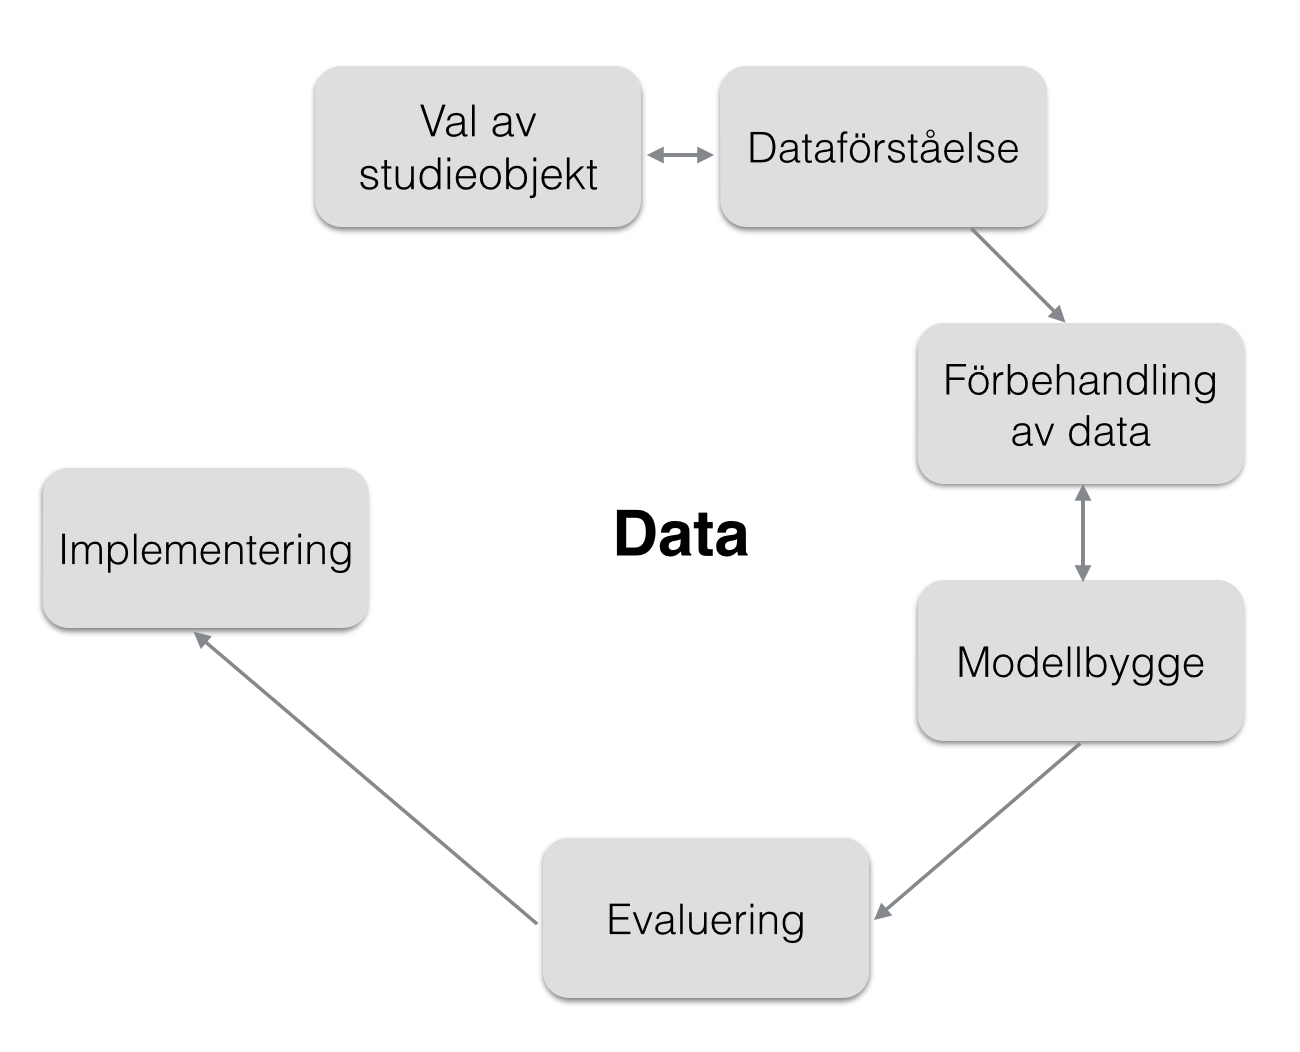
\includegraphics[width=0.8\textwidth]{Data.png}
\captionof{figure}{Experimentdesign}
\label{fig:design}            
\end{minipage}
\\

Implementeringen består av en case-mix-justering som genomförs i tre steg: uppskattning av kontrollvariablers inverkan, generering av prediktion på patientnivå samt aggregering och justering på sjukhusnivå (Department of Health, 2012). En mer detaljerad beskrivning av case-mix-justeringen återfinns i avsnitt 4.6.

\subsection{Val av studieobjekt}

Den population som valts som objekt i denna studie är hjärtinfarktpatienter vid Karolinska sjukhuset i Solna och Huddinge. Det finns flera anledningar till valet av population. Då en del av syftet är att studera värdeskapande är det en fördel att studera en vårdgivare som arbetar med implementeringen av VBV. Då syftet också är att jämföra två enheter lämpar sig Karolinska bra då de Karolinska har två universitetssjukhus, som just för hjärtinfarkter visat sig ha skillnad i överlevnads statistik (Hälso- och sjukvård, 2013).

Som tidigare redogjorts för i teorikapitlet är det långt ifrån självklart hur ett arbete av detta slag bör mäta värdeskapande. I detta arbete kommer dock kvalitet att mäts genom utfallsmåttet “30 dagars mortalitet” och kostnaden genom att summera alla de kostnader hos patienten som kan kopplas till hjärtinfarkten. Valet gjordes i samråd med Erik Wiklund, chef över kvantitativ analys på Karolinska. Att istället för utfallsmått använda processmått hade varit enklare statistiskt men eftersom en del av syftet är att se hur populationsegenskaperna påverkar utfallet faller det sig naturligt att använda ett utfallsmått. Utfallsmåttet belyser också patientvärdet tydligare än processmått (Porter, 2010) vilket är en stark anledning att man väljer att styra enligt VBV för att komma till rätta med kritiken mot NPM. Måttet ``30 dagars mortalitet'' är ett av de mest förekommande utfallsmåtten som används i Sverige idag (Wiklund, 2015) och är extra intressant eftersom de två enheterna (Solna och Huddinge) presterat över respektive under rikssnittet för dessa mått (Hälsa och Sjukvård, 2013). En viktig del i metodvalet för detta arbete har varit att bestämma hur kvalitetskapandet mäts. Porter (2010) hävdar att kvalitet bör ses som summan av alla utfall hos patienten, något som anses ge en mer komplett bild av värdeskapandet. Nordenström anser emellertid att processmått också innehåller viktig information om värdeskapande(Nordenström, 2014). Valet av kvalitetsmått skulle i detta arbetet kunnat göras annorlunda, något som kan påverka studiens resultat.

Det är viktigt att ha i åtanke att ingen information om dödsorsak erhållits, det är således inte säkert att hjärtinfarkten i fråga lett till dödsfall hos de patienter som avlidit inom 30 dagar efter att de behandlats för hjärtinfarkt. Information om dödsorsak hos patienterna finns inte tillgänglig, vilket är en nackdel då det hade kunnat öka undersökningens validitet.

Det är även möjligt att Karoliskas två studerade patientpopulationer har mindre diversitet än två sjukhus från mer geografiskt skilda områden. Detta är dock något som ligger utanför omfånget hos denna studie.

\subsection{Datainsamling}

Data som används har erhållits från Sektionen för Strategiska projekt, analys och visualisering vid Karolinska Sjukhuset. Patienterna hämtades från ett kvalitetsregister och innehåller alla de patienter som lagts in för vård av hjärtinfarkt under kalenderåret 2013, totalt 1190 patienter. Kvalitetsregistret innehåller bland annat biometrisk information samt mortalitet för olika tidshorisonter efter behandling. Dessa patienters kompletta vårdhistorik har funnits att tillgå via ett vårdhistoriksregister som innehåller infomation om alla vårdkontakter patienten haft. Det utdrag som erhållits består av utdrag från vårdhistoriksregistret ett år före hjärtinfarkten till ett år efter, totalt innehåller registret data information om 19684 vårdtillfällen. Vårdhistoriksregistret innehåller information om var patienten behandlats, av vilken anledning samt till vilken kostnad. Data från Karolinska har även kompletterats med socioekonomiska variabler då dessa i tidigare rapporter visat sig påverka risken för hjärtinfarkt (Chaix et al., 2007). Socioekonomisk data har hämtats från Statistiska centralbyrån (2013) och innehåller information om medelinkomst samt medelutbildningsnivå för olika postnummer. Det hade varit önskvärt att ha tillgång till data på individnivå föra att öka validiteten men då denna information inte funnits att tillgå har de socio-ekonomiska parametrarna skattats till medelvärdet för individernas postnummer.

Då datan innehåller patientdata på personnivå kan det vara känslig information för de berörda individerna (Sekaran, 2003, s. 51). Därför är patienternas personnummer krypterade för att öka individens integritet. I denna rapport kommer heller ingen information rörande specifika vårdfall publiceras med hänsyn till patienternas integritet.

\subsection{Förbehandling av data}

\subsubsection{Parametrar}


Vid genomförandet av en case-mix justering är en viktig del att välja vilka parametrar som inkluderas i modellbygget. Endast variabler som tros ha medicinsk signifikans bör inkluderas i modelleringen (Department of Health, 2012, s.7). De parametrar som valts ut till detta arbete har baserats på litteraturstudier inom området. Parametrarna finns presenterade i Tabell \ref{tab:raw1} och \ref{tab:raw2}, där även beskrivande statistik och antal saknade värden finns att tillgå.

Bara parametrar som tros vara medicinsk signifikanta har tagits med i modellbygget. Initialt har parametrar som i Hjärt- och lungfondens rapport “Hjärtinfarkt” beskrivs som riskfaktorer för hjärtinfarkt inkluderats, detta inkluderar parametrar såsom, rökning, hypertoni (högt blodtryck), hyperlidemi (höga blodfetter), övervikt (högt BMI) samt diabetes (Hjärt-Lungfonden, 2013). Även snusning lyfts i vissa rapporter fram som en riskfaktor (Bolinder, 2006). Som tidigare nämnts finns också korrelationer mellan risken att drabbas för hjärtinfarkt och en patients socio-ekonomiska situation och därför har parametrar som utbildningsnivå och medelinkomst i patientens kommun inkluderats (Chaix et al., 2007).

Däremot visade det sig vid en jämförelse av utbildningsnivå och medelinkomst att dessa två variabler, föga förvånande, korrelerade starkt. Därför togs beslutet att endast använda medelinkomst i modelleringen.

Varje vårdhändelse i vårdhistorikregistret hade en tillhörande kostnad vilka aggregerades för att ta fram kostnad per patient. Kostnaden har beräknats genom att för alla patienter ta med alla typer av kostnader som går att relatera till hjärtinfarkten vilket inkluderar; operationskostnader, återbesök, medicinering etc. Att summera alla de kostnader som är relaterade till just hjärtinfarkten gjordes genom att alla vårdhändelser som är markerade som indexhändelse (Första inläggningen för hjärtinfarkt) eller där händelsen är markerad med en “Akut hjärtinfarkt” eller “Hjärtinfarkt”. Noterbart är att andra följdkostnader som inte är markerade som hjärtinfarkt i vårdhistoriksregistret men ändå kan vara knutna till hjärtinfarkten inte kunnat inkluderas.


Den data som används består av både kategorivariabler och mätvariabler. Exempel på
kategorivariabel är “Sysselsättning” som består av ett begränsat antal
kategorier och således mäts på nomialskala. “Ålder vid ankomstdatum” är ett
exempel på en mätvariabel som anger hur mycket eller lite av en viss egenskap en
viss observation har, i detta fall ålder. Typ av variabel påverkar både dess
beskrivande statistik och hur de kan användas i en modell (Edling \& Hedström,
2003, s. 17). Det går till exempel inte att tala om medelvärde eller
standardavvikelse för en kategorivariabel och för att använda dem i en modell krävs att de dummykodas (Edling \& Hedström, 2003, s. 53 \& 102).

\begin{table}[htbp]
\centering
\caption{Obehandlade mätvariabler}
\label{tab:raw1}    
{\footnotesize
\begin{tabular}{lrrrrrr}
 \textbf{Variabel} & $\mathbf{Antal}$ & \textbf{Min} & \textbf{Max} & $\mathbf{\bar{x}}$ & $\mathbf{std.av.}$ & \textbf{Saknade} \\ 
  \hline
Ålder vid ankomstdatum & 1187 &     33.0 &     103.0 &     68.2 &     12.7 &  3 \\ 
  BMI & 1122 &     14.0 &     244.0 &     27.3 &      7.9 & 68 \\ 
  Antal diagnoser & 1190 &      1.0 &      14.0 &      2.9 &      1.8 &  0 \\ 
  Medelinkomst & 1168 & 203287.1 &  563920.6 & 259898.6 &  37659.3 & 22 \\ 
  % Utskrivningsenhet & 1190 &  10013.0 &   11002.0 &  10994.8 &     80.8 &  0 \\ 
  Kostnad per patient & 1190 &   5037.9 & 2255458.4 & 119623.0 & 133542.2 &  0 \\ 
  \end{tabular}
}
\end{table}

\begin{table}[htbp]
\centering
\caption{Obehandlade kategorivariabler} 
\label{tab:raw2}
{\footnotesize
\begin{tabular}{ll|rr}
 \textbf{Variabel} & \textbf{Värde} & $\mathbf{Antal}$ & $\mathbf{\%}$ \\ 
  \hline
Kön & Kvinna & 334 & 28.1 \\ 
   & Man & 856 & 71.9 \\ 
   \hline
 & Samtliga & 1190 & 100.0 \\ 
   \hline
\hline
Sysselsättning & Arbete & 290 & 24.4 \\ 
   & Arbetslöshet & 23 & 1.9 \\ 
   & Pensionär & 714 & 60.0 \\ 
   & Sjukskrivning & 31 & 2.6 \\ 
   & Studier/Övrigt & 8 & 0.7 \\ 
   & Saknade & 124 & 10.4 \\ 
   \hline
 & Samtliga & 1190 & 100.0 \\ 
   \hline
\hline
Rökning & Aldrig rökare & 428 & 36.0 \\ 
   & Ex-rökare \textgreater 1 mån & 324 & 27.2 \\ 
   & Rökare & 296 & 24.9 \\ 
   & Saknade & 142 & 11.9 \\ 
   \hline
 & Samtliga & 1190 & 100.0 \\ 
   \hline
\hline
Snusning & Aldrig varit snusare & 796 & 66.9 \\ 
   & Ex-snusare \textgreater 1 mån & 19 & 1.6 \\ 
   & Snusare & 55 & 4.6 \\ 
   & Saknade & 320 & 26.9 \\ 
   \hline
 & Samtliga & 1190 & 100.0 \\ 
   \hline
\hline
Tidigare.hjärtinfarkt & Ja & 319 & 26.8 \\ 
   & Nej & 855 & 71.8 \\ 
   & Saknade & 16 & 1.3 \\ 
   \hline
 & Samtliga & 1190 & 100.0 \\ 
   \hline
\hline
Diabetes & Ja & 290 & 24.4 \\ 
   & Nej & 895 & 75.2 \\ 
   & Saknade & 5 & 0.4 \\ 
   \hline
 & Samtliga & 1190 & 100.0 \\ 
   \hline
\hline
Hypertoni & Ja & 586 & 49.2 \\ 
   & Nej & 595 & 50.0 \\ 
   & Saknade & 9 & 0.8 \\ 
   \hline
 & Samtliga & 1190 & 100.0 \\ 
   \hline
\hline
Tablettbehandlad.hyperlipedemi & Ja & 360 & 30.2 \\ 
   & Nej & 818 & 68.7 \\ 
   & Saknade & 12 & 1.0 \\ 
   \hline
 & Samtliga & 1190 & 100.0 \\ 
   \hline
\hline
Död.30dgr & Ja & 88 & 7.4 \\ 
   & Nej & 1082 & 90.9 \\ 
   & Saknade & 20 & 1.7 \\ 
   \hline
 & Samtliga & 1190 & 100.0 \\ 
   \hline
\hline
Utskr\_Inr & Övriga & 8 & 0.7 \\ 
   & Solna & 653 & 54.9 \\ 
   & Huddinge & 529 & 44.5 \\ 
   \hline
 & Samtliga & 1190 & 100.0 \\ 
   \hline
\hline
\end{tabular}
}

\end{table}


\subsubsection{Saknade eller okända värden}
Ett problem inför modelleringen var att behandla saknade värden. Som framgår i Tabell \ref{tab:raw1} och \ref{tab:raw2} saknades värden på flertalet variabler. Till att börja med saknades information om “30 dagars mortalitet” för 20 av patienterna. Dessa 20 patienter togs bort då “30 dagars mortalitet” är målvariabel i modellen och dessa data således inte kan användas. Dessutom var det 8 patienter som hade skrivits ut från en annan vårdenhet än Solna eller Huddinge, även dessa 8 togs bort då de inte tillför något i jämförelsen. Efter att dessa individer  tagits bort reducerades datamängden från 1190 patienter till 1162.

Flera av de parametrar som ansågs viktiga för modelleringen innehöll  saknade värden. Dessvärre var det även en större mängd av de parametrar som ansågs vara av intresse för modellen som innehöll saknade värden eller okända värden. Om alla de patienter med saknade eller okända värden i de utvalda fälten skulle tagits bort hade populationen reducerats från 1162 till 733, se Tabell \ref{tab:raw1} och \ref{tab:raw2}. För att undvika detta gjordes en bootstrap för de saknade och okända fälten. Detta gjordes genom att ersätta de saknade och okända fälten med nya värden samplade ur fördelningen av de kända värdena från samma fält (Efron, 1994). Ett komplett dataset hade varit önskvärt, då det hade inneburit en högre reabilitet. Ett alternativ till bootstrap hade varit att helt enkelt utesluta alla patienter där ett eller flera värden saknas, dock hade detta också minskat reabiliteten då helhetsbilden rubbas. 

Till skillnad från andra liknande studier har saknade värden i detta arbete genererats med hjälp av bootstrap istället för att tas bort. Anledningen till detta är att vår studerade population varit betydligt mindre och att bortfallet av patienter hade skiljt sig betydligt mellan de två studerade enheterna. Värt att notera är att, enligt överläkare Thomas Järnberg,  har ofta patienter med mer komplexa sjukdomsbilder fler saknade värden. Detta faktum tillsammans med att andel saknade värden skiljde sig åt mellan de två vårdenheterna är anledningen till att bootstrap använts i detta arbete.

\subsubsection{Felregistrerade värden och omkodning av variabler}
I ett tidigt skede upptäcktes vissa extremvärden som kraftigt avvek från vad som ansågs vara rimligt. Detta var färmst för BMI där en patient hade ett registrerat BMI på 244 och en hade 53. För att bekräfta att det i dessa fall rörde sig om en felregistrering bekräftades BMI-registreringarna genom att studera längd och vikt för patienterna. Dessa värden togs bort och bootstrapp användes igen för att fylla dessa värden. Flera patienter uppvisade kostnader långt högre än genomsnitten, det största var 2,25 mkr i förhållande till genomsnitten på 120 tkr. Dessa tilläts dock vara kvar då de ansågs korrekta.

Vissa av parametrarna, exempelvis “Ex-snusare \textgreater1 mån” i fältet “Snusare” och “Studier/Övrigt” i fältet Sysselsättning förekom väldigt sällan i förhållande till hela datat, 1,6 respektive 0,7 \% av populationen. För att undvika att variansen för dessa variabler blev orimligt hög kodades de om. “Ex-snusare \textgreater1 mån” kodades om till “Snusare” och för att vara konsekvent gjordes även motsvarande för “Ex-rökare \textgreater1 mån”. Under Sysselsättning gjordes en likande omkodning där “Arbetslöshet”, “Sjukskrivning” och “Studier/Övrigt” alla kodades om till den nya kategorien “Övrigt”.

\subsection{Datautforskning}

Det första steget i datautforskningen var att studera den beskrivande statistiken för all data, uppdelat på de patienter som avlidit inom 30 dagar från första besöket och de som inte gjort det. Detta finns presenterat i Tabell \ref{tab:dl1} och Tabell \ref{tab:dl2}. Det går att utläsa skillnader i variabler som påverkar sannolikheten att överleva. Exempelvis framgår i Tabell \ref{tab:dl1} att genomsnittlig “Ålder vid ankomstdatum” skiljer sig markant mellan de två grupperna. De som avlider i genomsnitt är 78,1 år vid ankomst medan de som överlever är 67,5 år. Detta är en indikation på att “Ålder vid ankomstdatum” kommer att ha en en viss förklaringsgrad i modellen, vilket också förväntas baserat på de studier som ligger till grund för dataurvalet. Även Sysselsättning “Pensionär” är överrepresenterad bland de som avlidit. 90 \% av de som avlidit var pensionärer trots att denna grupp endast stod för 66 \% av hela patientpopulationen. Detta ligger i linje med att ålder kraftigt påverkar sannolikheten att överleva en hjärtinfarkt. Andra signifikanta skillnader som ligger i linje med resultaten av Hjärt-Lungfondens studie är att “Antal diagnoser”, “Diabetes” och “Hypertoni” påverkar överlevnadssannolikheten negativt. Däremot är det svårt att utläsa någon effekt av “Snusning”, “Rökning” och “Medelinkomst”. Motsatt mot vad som sägs i Hjärt-Lungfondens studie om risken ett drabbas av hjärtinfarkt tycks ett högre BMI öka chansen att överleva en hjärtinfarkt i detta arbete. Kostnaden för patienter som avlidit är något högre än för de som överlever, 146,3 tkr jämfört med 117,3 tkr, däremot har gruppen som avlidit högre standardavvikelse.

\begin{table}[htbp]
\centering
\caption{Mätvariabler uppdelat på ''Död 30 dagar'' Ja/Nej}
\label{tab:dl1}
{\footnotesize
\begin{tabular}{llrrrrr}
 \textbf{Variabel} & \textbf{Värde} & $\mathbf{n}$ & \textbf{Min} & \textbf{Max} & $\mathbf{\bar{x}}$ & $\mathbf{std.av.}$ \\ 
  \hline
Ålder vid ankomstdatum & Ja &   86 &  49.0 &   95.0 &  78.1 &  10.6 \\ 
   & Nej & 1076 &  33.0 &   98.0 &  67.5 &  12.4 \\ 
   \hline
 & Samtliga & 1162 &  33.0 &   98.0 &  68.2 &  12.6 \\ 
   \hline
BMI & Ja &   86 &  14.0 &   38.0 &  24.5 &   3.8 \\ 
   & Nej & 1076 &  14.0 &   45.0 &  27.3 &   4.4 \\ 
   \hline
 & Samtliga & 1162 &  14.0 &   45.0 &  27.1 &   4.4 \\ 
   \hline
Antal diagnoser & Ja &   86 &   1.0 &    9.0 &   3.5 &   2.0 \\ 
   & Nej & 1076 &   1.0 &   13.0 &   2.9 &   1.8 \\ 
   \hline
 & Samtliga & 1162 &   1.0 &   13.0 &   2.9 &   1.8 \\ 
   \hline
Medelinkomst & Ja &   86 & 211.2 &  332.7 & 266.7 &  35.7 \\ 
   & Nej & 1076 & 203.3 &  399.9 & 258.9 &  36.5 \\ 
   \hline
 & Samtliga & 1162 & 203.3 &  399.9 & 259.5 &  36.5 \\ 
   \hline
Kostnad per patient & Ja &   86 &   5.0 & 1178.1 & 146.3 & 191.4 \\ 
   & Nej & 1076 &  10.4 & 2255.5 & 117.3 & 126.9 \\ 
   \hline
 & Samtliga & 1162 &   5.0 & 2255.5 & 119.4 & 132.9 \\ 
   \hline
\end{tabular}
}
\end{table}


\begin{table}[htbp]
\centering
\caption{Kategorivariabler uppdelat på ''Död 30 dagar'' Ja/Nej}
\label{tab:dl2}
{\footnotesize
\begin{tabular}{ll|rr|rr|rr}
 \textbf{Variabel} & \textbf{Värde} & $\mathbf{n_{\mathrm{Ja}}}$ & $\mathbf{\%_{\mathrm{Ja}}}$ & $\mathbf{n_{\mathrm{Nej}}}$ & $\mathbf{\%_{\mathrm{Nej}}}$ & $\mathbf{n_{\mathrm{all}}}$ & $\mathbf{\%_{\mathrm{all}}}$ \\ 
  \hline
Kön & Kvinna & 27 & 31.4 & 299 & 27.8 & 326 & 28.1 \\ 
   & Man & 59 & 68.6 & 777 & 72.2 & 836 & 71.9 \\ 
   \hline
 & Samtliga & 86 & 100.0 & 1076 & 100.0 & 1162 & 100.0 \\ 
   \hline
\hline
Sysselsättning & Arbete & 3 & 3.5 & 321 & 29.8 & 324 & 27.9 \\ 
   & Pensionär & 80 & 93.0 & 688 & 63.9 & 768 & 66.1 \\ 
   & Övrigt & 3 & 3.5 & 67 & 6.2 & 70 & 6.0 \\ 
   \hline
 & Samtliga & 86 & 100.0 & 1076 & 100.0 & 1162 & 100.0 \\ 
   \hline
\hline
Rökning & Aldrig rökare & 36 & 41.9 & 440 & 40.9 & 476 & 41.0 \\ 
   & Rökare & 50 & 58.1 & 636 & 59.1 & 686 & 59.0 \\ 
   \hline
 & Samtliga & 86 & 100.0 & 1076 & 100.0 & 1162 & 100.0 \\ 
   \hline
\hline
Snusning & Aldrig varit snusare & 83 & 96.5 & 983 & 91.4 & 1066 & 91.7 \\ 
   & Snusare & 3 & 3.5 & 93 & 8.6 & 96 & 8.3 \\ 
   \hline
 & Samtliga & 86 & 100.0 & 1076 & 100.0 & 1162 & 100.0 \\ 
   \hline
\hline
Tidigare hjärtinfarkt & Ja & 30 & 34.9 & 283 & 26.3 & 313 & 26.9 \\ 
   & Nej & 56 & 65.1 & 793 & 73.7 & 849 & 73.1 \\ 
   \hline
 & Samtliga & 86 & 100.0 & 1076 & 100.0 & 1162 & 100.0 \\ 
   \hline
\hline
Diabetes & Ja & 30 & 34.9 & 255 & 23.7 & 285 & 24.5 \\ 
   & Nej & 56 & 65.1 & 821 & 76.3 & 877 & 75.5 \\ 
   \hline
 & Samtliga & 86 & 100.0 & 1076 & 100.0 & 1162 & 100.0 \\ 
   \hline
\hline
Hypertoni & Ja & 50 & 58.1 & 531 & 49.4 & 581 & 50.0 \\ 
   & Nej & 36 & 41.9 & 545 & 50.6 & 581 & 50.0 \\ 
   \hline
 & Samtliga & 86 & 100.0 & 1076 & 100.0 & 1162 & 100.0 \\ 
   \hline
\hline
Tablettbehandlad hyperlipedemi & Ja & 25 & 29.1 & 335 & 31.1 & 360 & 31.0 \\ 
   & Nej & 61 & 70.9 & 741 & 68.9 & 802 & 69.0 \\ 
   \hline
 & Samtliga & 86 & 100.0 & 1076 & 100.0 & 1162 & 100.0 \\ 
   \hline
\hline
Utskr\_Inr & Solna & 45 & 52.3 & 593 & 55.1 & 638 & 54.9 \\ 
   & Huddinge & 41 & 47.7 & 483 & 44.9 & 524 & 45.1 \\ 
   \hline
 & Samtliga & 86 & 100.0 & 1076 & 100.0 & 1162 & 100.0 \\ 
   \hline
\hline
Död 30 dagar & Ja & 86 & 100.0 & 0 & 0.0 & 86 & 7.4 \\ 
   & Nej & 0 & 0.0 & 1076 & 100.0 & 1076 & 92.6 \\ 
   \hline
 & Samtliga & 86 & 100.0 & 1076 & 100.0 & 1162 & 100.0 \\ 
   \hline
\hline
\end{tabular}
}
\end{table}

\begin{table}[htbp]
\centering
\caption{Mätvariabler uppdelat på Sjukhus} 
\label{tab:sh1}
{\footnotesize
\begin{tabular}{llrrrrr}
 \textbf{Variabel} & \textbf{Värde} & $\mathbf{n}$ & \textbf{Min} & \textbf{Max} & $\mathbf{\bar{x}}$ & $\mathbf{std.av.}$ \\ 
  \hline
Ålder vid ankomstdatum & Solna &  638 &  33.0 &   98.0 &  67.8 &  12.3 \\ 
   & Huddinge &  524 &  34.0 &   95.0 &  68.8 &  12.9 \\ 
   \hline
 & Samtliga & 1162 &  33.0 &   98.0 &  68.2 &  12.6 \\ 
   \hline
BMI & Solna &  638 &  14.0 &   42.0 &  27.0 &   4.2 \\ 
   & Huddinge &  524 &  14.0 &   45.0 &  27.2 &   4.7 \\ 
   \hline
 & Samtliga & 1162 &  14.0 &   45.0 &  27.1 &   4.4 \\ 
   \hline
Antal diagnoser & Solna &  638 &   1.0 &   10.0 &   2.7 &   1.6 \\ 
   & Huddinge &  524 &   1.0 &   13.0 &   3.2 &   2.1 \\ 
   \hline
 & Samtliga & 1162 &   1.0 &   13.0 &   2.9 &   1.8 \\ 
   \hline
Medelinkomst & Solna &  638 & 203.3 &  399.9 & 264.2 &  36.9 \\ 
   & Huddinge &  524 & 211.2 &  332.7 & 253.7 &  35.2 \\ 
   \hline
 & Samtliga & 1162 & 203.3 &  399.9 & 259.5 &  36.5 \\ 
   \hline
Kostnad per patient & Solna &  638 &   5.0 & 2255.5 & 115.6 & 145.0 \\ 
   & Huddinge &  524 &   8.8 & 1178.1 & 124.2 & 116.4 \\ 
   \hline
 & Samtliga & 1162 &   5.0 & 2255.5 & 119.4 & 132.9 \\ 
   \hline
\end{tabular}
}

\end{table}

\begin{table}[htbp]
\centering
\caption{Kategorivariabler uppdelat på Sjukhus} 
\label{tab:sh2}
{\footnotesize
\begin{tabular}{ll|rr|rr|rr}
 \textbf{Variabel} & \textbf{Värde} & $\mathbf{n_{\mathrm{Solna}}}$ & $\mathbf{\%_{\mathrm{Solna}}}$ & $\mathbf{n_{\mathrm{Huddinge}}}$ & $\mathbf{\%_{\mathrm{Huddinge}}}$ & $\mathbf{n_{\mathrm{Samtliga}}}$ & $\mathbf{\%_{\mathrm{Samtliga}}}$ \\ 
  \hline
Kön & Kvinna & 169 & 26.5 & 157 & 30.0 & 326 & 28.1 \\ 
   & Man & 469 & 73.5 & 367 & 70.0 & 836 & 71.9 \\ 
   \hline
 & Samtliga & 638 & 100.0 & 524 & 100.0 & 1162 & 100.0 \\ 
   \hline
\hline
Sysselsättning & Arbete & 190 & 29.8 & 134 & 25.6 & 324 & 27.9 \\ 
   & Pensionär & 411 & 64.4 & 357 & 68.1 & 768 & 66.1 \\ 
   & Övrigt & 37 & 5.8 & 33 & 6.3 & 70 & 6.0 \\ 
   \hline
 & Samtliga & 638 & 100.0 & 524 & 100.0 & 1162 & 100.0 \\ 
   \hline
\hline
Rökning & Aldrig rökare & 273 & 42.8 & 203 & 38.7 & 476 & 41.0 \\ 
   & Rökare & 365 & 57.2 & 321 & 61.3 & 686 & 59.0 \\ 
   \hline
 & Samtliga & 638 & 100.0 & 524 & 100.0 & 1162 & 100.0 \\ 
   \hline
\hline
Snusning & Aldrig varit snusare & 592 & 92.8 & 474 & 90.5 & 1066 & 91.7 \\ 
   & Snusare & 46 & 7.2 & 50 & 9.5 & 96 & 8.3 \\ 
   \hline
 & Samtliga & 638 & 100.0 & 524 & 100.0 & 1162 & 100.0 \\ 
   \hline
\hline
Tidigare hjärtinfarkt & Ja & 153 & 24.0 & 160 & 30.5 & 313 & 26.9 \\ 
   & Nej & 485 & 76.0 & 364 & 69.5 & 849 & 73.1 \\ 
   \hline
 & Samtliga & 638 & 100.0 & 524 & 100.0 & 1162 & 100.0 \\ 
   \hline
\hline
Diabetes & Ja & 134 & 21.0 & 151 & 28.8 & 285 & 24.5 \\ 
   & Nej & 504 & 79.0 & 373 & 71.2 & 877 & 75.5 \\ 
   \hline
 & Samtliga & 638 & 100.0 & 524 & 100.0 & 1162 & 100.0 \\ 
   \hline
\hline
Hypertoni & Ja & 291 & 45.6 & 290 & 55.3 & 581 & 50.0 \\ 
   & Nej & 347 & 54.4 & 234 & 44.7 & 581 & 50.0 \\ 
   \hline
 & Samtliga & 638 & 100.0 & 524 & 100.0 & 1162 & 100.0 \\ 
   \hline
\hline
Tablettbehandlad hyperlipedemi & Ja & 173 & 27.1 & 187 & 35.7 & 360 & 31.0 \\ 
   & Nej & 465 & 72.9 & 337 & 64.3 & 802 & 69.0 \\ 
   \hline
 & Samtliga & 638 & 100.0 & 524 & 100.0 & 1162 & 100.0 \\ 
   \hline
\hline
Utskrivningsenhet & Solna & 638 & 100.0 & 0 & 0.0 & 638 & 54.9 \\ 
   & Huddinge & 0 & 0.0 & 524 & 100.0 & 524 & 45.1 \\ 
   \hline
 & Samtliga & 638 & 100.0 & 524 & 100.0 & 1162 & 100.0 \\ 
   \hline
\hline
Död.30dgr & Ja & 45 & 7.0 & 41 & 7.8 & 86 & 7.4 \\ 
   & Nej & 593 & 93.0 & 483 & 92.2 & 1076 & 92.6 \\ 
   \hline
 & Samtliga & 638 & 100.0 & 524 & 100.0 & 1162 & 100.0 \\ 
   \hline
\hline
\end{tabular}
}

\end{table}


I Tabell \ref{tab:sh1} och \ref{tab:sh2} presenteras beskrivande statistik för all data, uppdelat på vårdenheterna Solna och Huddinge. Vid första anblick tycks det inte vara någon skillnad på “Ålder vid ankomstdatum” mellan de två vårdenheterna, detta är däremot inte hela sanningen. Om fördelningen av “Ålder vid ankomstdatum” jämförs, se Figur \ref{fig:alder}, går det att se att Huddinge har en större andel patienter som var över 78 år vid ankomstdatum. Huddinge har även ett högre genomsnitt på “Antal diagnoser” samt större andel med “Tidigare hjärtinfarkt”, “Diabetes”, “Hypertoni” och “Tabellbehandlad hyperlidemi”. Vad gäller den socioekonomiska parametern, ``Medelinkomst'', har patienterna vid Solna något högre värde än i Huddinge.

Till skillnad mot resultaten av Socialstyrelsens Öppna Jämförelse, som grundar sig i data fram till och med 2012, har Solna en lägre mortalitetsgrad än Huddinge. Solna har en lägre genomsnittlig kostnad än Huddinge och har därmed ett högre ojusterat värdeskapande. I Figur \label{fig:kostnad} går det att se tydligare att Huddinge har en högre andel patienter med hög kostnad.

\noindent\begin{minipage}{\textwidth}
\centering
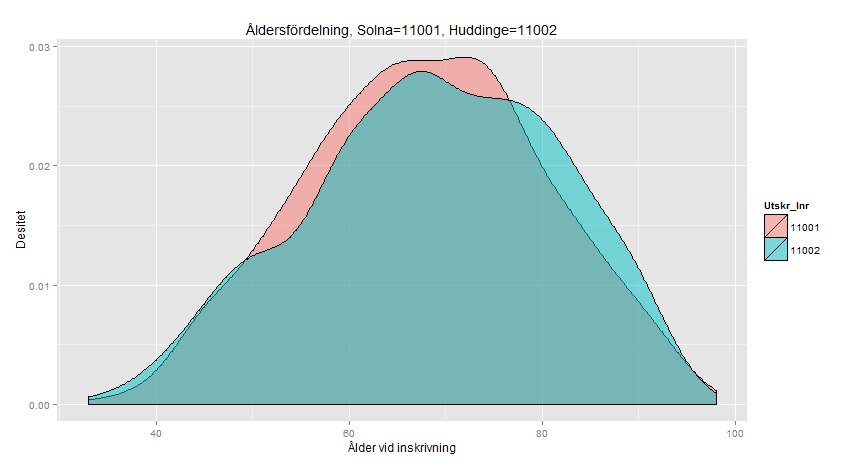
\includegraphics[width=1\textwidth]{alder.png}
\captionof{figure}{Åldersfördelning}
\label{fig:alder}            
\end{minipage}
\\

\noindent\begin{minipage}{\textwidth}
\centering
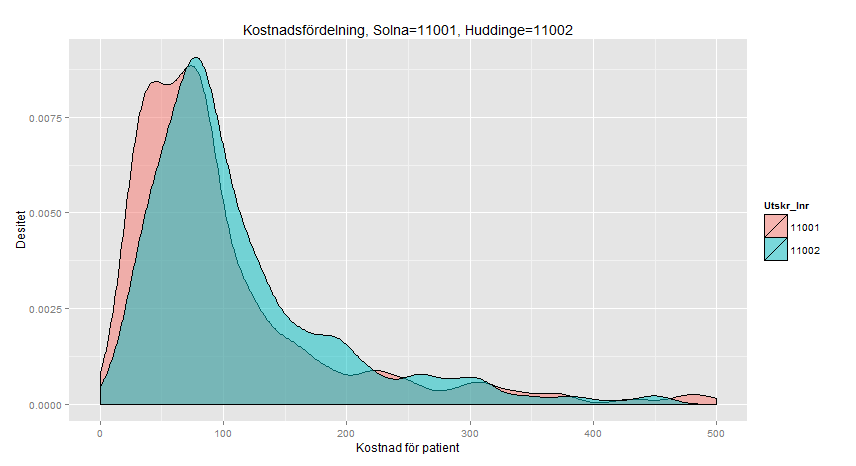
\includegraphics[width=1\textwidth]{kostnad.png}
\captionof{figure}{Kostnadsfördelning}
\label{fig:kostnad}            
\end{minipage}
\\

\subsection{Modellbygge}

För att kunna jämföra värdeskapandet mellan de två avdelningarna har tre modeller skapats för kvalitet samt tre modeller för kostnad. I samråd med Lars Lindhagen, biostatistiker som jobbat med liknande analyser av hjärtpatienter, beslutades att skapa tre modeller vilka skiljer sig åt genom att olika parametrar tagits med. De variabler som inkluderas i en case-mix-modell skall tros ha både medicinsk signifikans samt ha bevisad statistisk signifikans (Nelson, 2014 s. 16-19). För att skapa de tre modellerna har antalet parametrar reducerats i två steg baserat på statistisk signifikans vilket illustreras i Appendix 1 och 2.

För att modellera kostnaden har linjär regression använts. Linjär regression används för att undersöka sambandet mellan en eller flera parametrar och en kontinuerlig målvariabel, vilket är fallet för just kostnad. Parametrarna får sedan olika vikter beroende på i vilken grad de påverkar responsvariabeln (Edling \& Hedström, 2003). Dessa tre modeller och dess tillhörande variabler visas i Appendix 2.

För att modellera kvaliteten kan inte linjär regression användas eftersom målvariabeln, “30 dagars mortalitet” är binär. Istället används här logistisk regression, en regressionsmodell vars prediktioner alltid faller inom det korrekta sannolikhetsintervallet [0-1]. Även vid logistisk regression får de förklarande variablerna olika vikter beroende på i vilken utsträckning de påverkar responsvariabeln (Edling \& Hedström, 2003). De tre modellerna och tillhörande variabler visas i Appendix 1. 

\subsection{Evaluering}

För att välja modell till case-mix-justeringen valdes i båda fallen modellen med lägst “Akaike Information Criteria” (AIC). Att mäta AIC är ett sätt att utvärdera och välja modell utifrån flera kandidatmodeller. AIC väger samman förklaringsgrad och komplexitet hos modellerna och beräknar ett värde där det är önskvärt att modellen har så lågt AIC som möjligt (Burnham \& Anderson, 2004). Prediktionsmodell har valts utifrån lägst AIC för både kostnad- och kvalitetsmodell. För kostnad innebar detta modell 2 i Appendix 2 och för kvalitet modell 2 i Appendix 1.

\subsection{Implementering}
%\label{sec:casemix}
% \subsubsection{Case/mix}

I implementeringen används de framtagna modellerna för kostnad och överlevnad för att prediktera dessa utfallsvariabler på patientnivå. För alla patienter aggregeras dessa prediktioner till vårdenhetsnivå, för att sedan användas i justeringen. 

Ett Relativt Utfallsmått (RU) (Ekvationsnummer 2 och \ref{eq:metod2}) skapas sedan genom att beräkna kvoten mellan det faktiska utfallet och modellens prediktion.

\begin{equation}
\label{eq:metod1}
	RU_i = Faktiskt \,\,  utfall \,\, patient \,\, i/Predikterat \,\, utfall \,\, patient \,\, i
\end{equation}

\begin{equation}
\label{eq:metod2}
	RU_{enhet} = \frac{1}{N} \sum_{i=1}^{N} RU_i
\end{equation}


RU illustrerar förhållandet mellan vårdenhetens utförande i relation till vad som kan förväntas av dem givet dess patientpopulation. Ett RU på 1,4 indikerar att vårdenheten har 40 procent högre resultat än vad som kan förväntas av dem givet den patientinformation som finns, medan 0,8 indikerar ett 20 procent lägre resultat (Department of Health, 2012).

Nästa steg i case-mix-justering är att göra själva justeringen. Detta görs genom att dividera de faktiska utfallet för vårdenheten med dess RU enligt (ekvationsnummer \ref{eq:metod3}). Det justerade utfallet blir en indikation på vilket utfall som kan väntats av vårdenheten, givet att de hade behandlat en standardpopulation. Grundtanken med case-mix är alltså att justera för effekter av att vårdenheterna har olika typer av patienter. Det är även möjligt att använda case-mix-justering för att beräkna vilket utfall som kan förväntas av vårdenheten givet den patientpopulation de faktiskt har, i detta fall multipliceras istället det faktiska utfallet med RU (Nelson, 2014 s. 16-19).

\begin{equation}
\label{eq:metod3}
	Justerad \,\, Utfall = Faktiskt \,\, Utfall/RU
\end{equation}


\section{Resultat - Jämförelse av värdeskapande}

\begin{table}[h]
\centering
\caption{Resultat för kvalitet}
\label{tab:kvalres}
\begin{tabular}{|p{2cm}|p{3cm}|p{1cm}|p{4cm}|p{2cm}|}
\hline
         & 30 dagars mortalitet (\%) & RU    & Justerad 30 dagars mortalitet (\%) & Skillnad (\%) \\ \hline
Solna    & 7,0                      & 0,969 & 7,3                               & 0,3          \\ \hline
Huddinge & 7,8                      & 1,037 & 7,5                               & -0,3         \\ \hline
\end{tabular}
\end{table}

\begin{table}[h]
\centering
\caption{Resultat för kostnad}
\label{tab:kostres}
\begin{tabular}{|p{2cm}|p{3cm}|p{1cm}|p{4cm}|p{2cm}|}
\hline
         & Medelkostnad (tkr) & RU    & Justerad medelkostnad\newline (tkr) & Skillnad (tkr) \\ \hline
Solna    & 115,6              & 0,975 & 118,5                       & 2,9            \\ \hline
Huddinge & 124,2              & 1,030 & 120,5                       & -3,7           \\ \hline
\end{tabular}
\end{table}

Som redovisats i teorikapitlet är det inte bara ett sjukhus verksamhet som påverkar utfallet av kostnad och kvalitet, utan även patientpopulationens egenskaper. Detta styrks även i de modeller som tagits fram i detta arbete. En komplett modellbeskrivning för samtliga parametrar och i vilken grad dessa påverkar kvalitet respektive kostnad återfinns i Appendix 1 respektive Appendix 2.

Det framgår i avsnitt 4.3.4. att de två olika sjukhusenheterna har olika egenskaper hos patientpopulationerna, vilket tyder på olika förutsättningar att leverera samma värdeskapande. För att jämföra värdeskapandet mellan dessa enheter blir det därför viktigt att case-mix-justera för dessa skillnader.

Kvaliteten som i detta arbete mäts genom 30 dagars mortalitet skiljer sig mellan de två enheterna, vilket presenteras i Tabell \label{tab:kvalres}. Innan case-mix-justeringen har Solna en lägre mortalitet (7,0 \%) jämfört med Huddinge (7,8 \%). I den framtagna modellen för att prediktera mortalitet är den klart mest bidragande faktorn hög ålder, en egenskap där populationen i Huddinge har ett högre medelvärde än Solna. Att Huddinge har en svårare population ur kvalitetssynpunkt syns i det relativa utfallet (1,037) jämfört med Solna (0,969). Att modellen ger ett RU mindre än 1 för Solna och ett RU över 1 för Huddinge indikerar att Solna presterar något under medan Huddinge presterar något över vad de förväntas, gällande mortalitetgivet dess patientpopulationer. Båda ligger däremot relativt nära 1 vilket tyder på att de båda vårdenheterna inte avviker nämnvärt. Kvalitetsskillnaden minskar efter case-mix-justeringen från 0,8 till 0,2 procentenheter. Case-mix-justering har således en neutraliserade effekt på kvalitetsskillnaden mellan de två sjukhusenheterna, och det är är svårt att utifrån detta arbete uttala sig som vilket sjukhus som producerar högst kvalitet. 

Även kostnaden skiljer sig åt mellan de de två enheterna vilket illustreras i Tabell \ref{tab:kostres}. Före justeringen genomförs har Huddinge en högre medelkostnad per patient (124,2 tkr) jämfört med Solna (115,6 tkr). I den framtagna modellen för att prediktera kostnad är de två mest bidragande parametrarna antal diagnoser och huruvida patienten har diabetes eller ej. Huddinge har generellt patienter med fler diagnoser samt större andel diabetiker vilket tyder på att de har svårare att producera med lägre kostnad. Att Huddinge har en dyrare patientpopulation syns i det relativa utfallet (1,030) jämfört med Solna (0,975). Även här är skillnaderna små, justerat för populationerna minskar skillnaden i medelkostnad från 8,6 tkr till 2,0 tkr. Case-mix-justeringen har därmed även en neutraliserande effekt på kostnadsskillnaden.

Att justeringen inte får större effekt kan bero på att de variabler som används vid modelleringen är baserade på studier för risken att få en hjärtinfarkt, inte risken att avlida av den eller kostnader associerade med behandlingen av den. En annan förklaring skulle kunna vara att populationerna är väldigt likartade, det hade därför varit intressant att jämföra med populationer från andra städer och länder.

Som tidigare nämnts är det enligt VBV eftersträvansvärt att skapa så hög kvalitet i förhållande till kostnad som möjligt. I denna rapport kan vi således definiera värde som överlevnad (\%) dividerat med kostnad (tkr). Värdeskapandet före och efter case-mix-justeringen visas i Tabell \ref{tab:varderes}.

\begin{table}[h]
\centering
\caption{Resultat för värdeskapande}
\label{tab:varderes}
\begin{tabular}{|p{4cm}|p{3cm}|p{2.5cm}|p{3.5cm}|}
\hline
Övelevnad (\%) / Kostnad (tkr)           & Värdeskapande innan case-mix & Värdeskapande efter case-mix & Case-mix påverkan på resultat \\ \hline
Solna                       & 0.8044                       & 0.7822                       & -0.0222                       \\ \hline
Huddinge                    & 0.7423                       & 0.7676                       & 0.0253                        \\ \hline
Skillnad mellan \linebreak vårdenheter & 0.0621                       & 0.0146                       &                               \\ \hline
\end{tabular}
\end{table}

\section{Diskussion}

Som redogjorts för i avsnitt 2 avser värdeskapande kvoten mellan kvalitet och kostnad. Det råder dock ingen konsensus om exakt hur kvalitet och kostnaden skall beräknas. Till exempel är inte Porter och Nordengren överens huruvida processmått, utfallsmått eller en kombination av dessa bör användas inom kvalitetsmätning. Något som krävs vid mätningen av kvalitet är att case-mix-justering används vilken avser att normera populationseffekterna. Även vid case-mix-justeringen saknas konsensus om vilka modeller och parametrar som bör användas.

Värdeskapande inom VBV har liknande grundtanke som värdeskapande inom verksamhetsstyrning. I verksamhetsstyrning utgår värdeskapandet från kunden medan detta inom VBV utgår ifrån patienten. En av de stora frågorna blir då om det går att se patienten som en kund, och om inte så är fallet, vad som skiljer dem åt. 

Vid genomförandet av den jämförande undersökningen har det framkommit att många val måste göras; val gällande hur kvalitet mäts, val gällande hur kostnad per patient beräknas samt val angående vilka statistiska modeller och parametrar som används. Dessa val hade i detta arbete kunnat ska på annat sett vilket hade kunnat generera andra resultat. För att göra dessa val krävs bland annat medicinsk kompetens, statistisk kompetens och ekonomisk kompetens.

Detta tillsammans med att ingen konsensus råder gällande dessa frågor visar på svårigheter med att jobba enligt VBV-konceptet. Just denna komplexitet är något som i problematiseringen lyfts fram som kritik mot konceptet, en bild som återspeglas i detta arbete.



NPM har växt fram som ett resultat av ett ökat kostnadsfokus, något som fått kritik är att patientfokuset blivit lidande. VBV har växt fram delvis som ett svar mot denna kritiken och erbjuder ett värdefokus som utgår ifrån patienten. Kan då VBV vara lösningen av de NPM-relaterade problemen? Tydligt är att VBV aspirerar på att komma tillrätta med det bortglömda patientfokuset. Det finns samtidigt många element som ingår i både NPM och VBV-begreppet såsom vikten att mäta, jämföra och kvantifiera. 






Om VBV skall lyckas komma tilrätta med den kritik som riktas mot NPM och uppnå önskat resultat, att maximera värdeskapandet utifrån patienten, krävs ett omfattande arbete. Om VBV skall kunna få full effekt krävs utredningar för framtagande och ramverk med tydliga instruktioner. Det vore också fruktbart att analysera effekterna av den VBV-implementering som i dagsläget sker inom svenska vårdenheter, dels gentemot vårdenheter med andra styrmodeller men också jämföra vården före och efter implementeringen.Det är tydligt att det vid en implementation av VBV blir det av stor vikt att utforma ramverk för hur mätningar sker och vilka avgränsningar som görs. I detta arbete har 


Troligtvis måste nya procedurer angående patientuppföljning skapas för att skapa en så komplett bild av den patientupplevda kvaliteten som möjligt.

 
Detta är ett viktigt och troligtvis mödosamt arbete som blir helt avgörande för det resultat implementationen uppnår.






Vilka svårigheter finns?


Vid jämförelse av värdeskapande mellan organisationer är det viktigt att justera för att dessa behandlar olika populationer och således har olika förutsättningar att producera samma värde. Även vid denna typen av justering är det avgörande vilka parametrar som inkluderas samt vilka metoder som används. Klinisk kunskap krävs för att bestämma vilka parametrar som tros vara kliniskt relevanta. Statistisk kunskap krävs för att avgöra de statiska modeller som används och undersöka vilka parametrar som är statistiskt signifikanta. Dessa val hade i detta arbete också kunnat ske på ett annat sätt vilket kunnat generera annorlunda resultat.

Detta arbete visar på svårigheterna både att mäta värde och att jämföra värde mellan enheter. Just denna komplexitet är något som lyfts fram som kritik mot VBV. Vissa hävdar att det är en omöjlighet att kunna utforma dessa mätningar på ett rättvist sätt och att VBV således blir en omöjlighet att implementera i praktiken.






Vad krävs för en lyckad implementering


De reformer som påverkat den svenska vård- och omsorgssektorn de senaste åren har lett till att sättet dessa organisationer styrs innehåller starka inslag av NPM. NPM har dock mött stark kritik från flera håll som grundar sig i att vårdorganisationer flyttat fokus från patienter och istället arbetar mot ekonomiska incitament. Dock är många överens om att vissa delar inom NPM kan vara fruktbara, framförallt gällande vikten av att mäta och målstyra verksamheten samt att möjliggöra jämförelser mellan organisationer.



Ett ökat patientfokus är något som framhålls som en av de stora förtjänsterna vid en implementation av VBV. Dock är det komplext att mäta det värdeskapande som är grundläggande vid VBV-styrning. Vilka parametrar som inkluderas i kvalitets- och kostnadsmåttet har stor effekt på utfallet av dessa och det råder ingen tydlig konsensus över hur dessa ramverk bör utformas. Porter (2010) menar exempelvis att kvalitet bör ses som summan av alla utfallsmått hos en patient medan processmått är mindre tillämpbara ur ett VBV-perspektiv eftersom dessa inte har ett lika tydligt patientfokus. Nordenström (2014) menar å andra sidan att processmått visst innehåller information som i högsta grad är relevant ur VBV-perspektivet. I detta arbete har kvalitet mätts genom mortalitet, ett utfallsmått som endast avser den högsta nivån av utfallsmått som presenteras i Tabell \label{tab:livslangd}. I en mer omfattande studie skulle fler parametrar, från samtliga nivåer, kunna inkluderas i kvalitetsmåttet för att skapa en mer komplett bild av värdeskapandet.




\section{Slutsats}

Syftet med detta arbete är att undersöka hur värdeskapande mäts inom VBV genom att jämföra värdeskapande mellan två vårdenheter på Karolinska. Det framgår att det finns skillnader i värdeskapandet där Solna har ett högre värdeskapande jämfört med Huddinge i det studerade exemplet. Skillnader finns också mellan de populationer vårdenheterna behandlar, som påverkar värdeskapandet, där Huddinge vårdar en svårare population. Justeringen för populationernas effekt har en neutraliserande inverkan på denna skillnad, dock uppnår Solna ett något högre värdeskapande även efter denna populationsjustering.

Att utforma en jämförelse av värdeskapande är svårt, då det inte råder någon konsensus om vilka parametrar och modeller som bör användas. Vid implementering av VBV blir således ett viktigt steg att utforma ramverk och procedurer för att mäta och jämföra värdeskapandet. 

\subsection{Framtida forskning}

Resultaten av detta arbete antyder att det finns behov av att flera saker undersöks närmre. Till att börja med finns det behov av vidare studier i hur ett värdemått konstrueras. Detta arbete har endast använt sig av ett utfallsmått och sannolikt krävs det en sammanvägning av flera för att skapa ett mer komplett värdemått, med fokus på patienten. Exempelvis skulle utfallsmått relaterade till patientens upplevda livskvalitet och bemötade inkluderas.

I vidare forskning krävs även för utformning av modeller för case-mix-justering. Parameterval i detta arbete har grundats på studier om risk att drabbas av hjärtinfarkt. Om flera utfallsmått ska vägas samman behöver justeringsmodeller för dessa mått även konstrueras. Detta kompliceras av att olika diagnoser kräver olika utfallsmått, vilket kommer att innebära att en stor mängd case-mix-modeller behöver konstrueras.

Gällande VBV finns det ännu inte mycket forskning på resultat av implementering under svenska förhållanden. Inom detta område finns det utrymme för en mängd forskning. Mest uppenbart vore att jämföra vården före och efter implementering. Då VBV gör anspråk på ökat patientfokus bör även detta beläggas med mer empiri innan fullskalig implementation påbörjas.

\section{Referenser}
\setlength{\parindent}{0cm}

\subsection{Publikationer}

Agevall, L. (2005). Välfärdens organisering och demokratin: en analys av New Public Management. Växjö: Växjö University Press\newline

Almqvist, RM. (2006). New public management: NPM : om konkurrensutsättning, kontrakt och kontroll. 1. uppl. Malmö: Liber		\newline
	
Arnek, M. (2013). Den offentliga sektorn: en antologi om att mäta produktivitet och prestationer. Stockholm: Finansdepartementet, Regeringskansliet\newline

Bolinder, G. (2006). All tobak ökar hjärtinfarktrisken: Snus ingen lösning för rökavvänjning. Läkartidningen nr 50–52 2006 volym 103\newline

Burnham, K. P., \& Anderson, D. R. (2004). Multimodel inference understanding AIC and BIC in model selection. Sociological methods \& research, 33(2), 261-304.\newline

Chaix, B., Rosvall, M., \& Merlo, J. (2007). Recent increase of neighborhood socioeconomic effects on ischemic heart disease mortality: a multilevel survival analysis of two large Swedish cohorts. American Journal of Epidemiology,165(1), 22-26.\newline

Chapman, P., et al. (2000). "CRISP-DM 1.0 Step-by-step data mining guide.".\newline

Department of Health. (2012). Patient Reported Outcome Measures (PROMs) in England: The case-mix adjustment methodology. Published to DH website, in electronic PDF format only.\newline

Edling, C. \& Hedström, P. (2003). Kvantitativa metoder: grundläggande analysmetoder för samhälls- och beteendevetare. Lund: Studentlitteratur\newline

Efron, B. (1994). Missing data, imputation, and the bootstrap. Journal of the American Statistical Association, 89(426), 463-475.\newline

Engström, I. (2014). NPM – en av de viktigaste frågorna. Läkartidningen. 2014;111:CPE9.\newline

Järhult, B., Secher, E., Akner, G. (2014). Värdebaserad vård lika illa som New public management. Läkartidningen. 2014;111:C77E\newline

Hjärt-Lungfonden. (2013). Hjärtinfarkt: En skrift om vad som händer under och efter infarkt. Stockholm.\newline

Hogstedt, Carl (2006). Medellivslängd och ohälsotal utmed spårtrafiken i Stockholm: hälsan på spåret. Stockholm: Statens folkhälsoinstitut\newline

Hood, C. (1991) "A public management for all seasons?." Public administration 69.1: 3-19.\newline

Hood, C. (1995). "The “New Public Management” in the 1980s: variations on a theme." Accounting, organizations and society 20.2: 93-109.\newline

Målqvist, I., Åborg, C., \& Forsman, M. (2011). Styrformer och arbetsförhållanden inom vård och omsorg–en kunskapssammanställning om New Public Management. Stockholm, Sweden: Institutionen för folkhälsovetenskap, Karolinska Institutet.\newline

Nelson, G. S. (2014) Reporting Healthcare Data: Understanding Rates and Adjustments.\newline

Nordenström, J. (2014) Värdebaserad vård kan ge bättre vårdutfall.  Läkartidningen. 2014;111:CZCR\newline

Nordenström, J. (2014). Värdebaserad vård: är vi så bra vi kan bli?. Stockholm: Karolinska institutet University Press\newline

Porter ME, Olmsted Teisberg E. (2006). Redefining health care: creating value-based competition on results. Boston: Harvard Business School Press\newline

Porter, ME, (2008). Competitive advantage: Creating and sustaining superior performance. Simon and Schuster. \newline

Porter, ME. (2010). "What is value in health care?." New England Journal of Medicine 363.26 (2010): 2477-2481.\newline

Uma, S., \& Roger, B. (2003). Research methods for business: A skill building approach. John Wiley and Sons Inc., New York.\newline

Waters, D., \& Waters, C. D. J. (2008). Quantitative methods for business. Pearson Education.\newline

Öppna jämförelser 2013. Hälso- och sjukvård : jämförelser mellan landsting. (2012). Stockholm: Sveriges kommuner och landsting.Tillgänglig på Internet: http://www.socialstyrelsen.se/publikationer2013/2013-12-1\newline

\subsection{Hemsidor}		 	 	 							

Dawson, J., Smith, L., Deubert, K. \& Grey-Smith, S. 2002. “S” Trek 6: referencing, not plagiarism. Retrieved October 31, 2002, from http://studytrekk.lis.curtin.edu.au/ \newline

DN. (2013). Den olönsamma patienten. Hämtad 2015-03-20, från http://www.dn.se/stories/stories-kultur/den-olonsamma-patienten/\newline

Forsberg, N., Magnusson, Ö., Olofsson, D. (2014). Nu har läkarna tröttnat på byråkratin, Hämtad 2015-04-03, från http://www.svt.se/agenda/lakarna-later-som-foretagsledare\newline
			
Karolinska. (2015). Fakta om sjukhuset. Hämtad: 2015-04-09, från http://www.karolinska.se/om-karolinska/Fakta-om-sjukhuset-Verksamhetsplaner--arsberattelsen--presentationsbroschyrer--organisation/\newline				

KDnuggets. (2007). Polls : Data Mining Methodology. Hämtad 2015-05-15,\newline från http://www.kdnuggets.com/polls/2007/data\_mining\_methodology.htm\newline

Nationella kvalitetsregister. (2014). Om Nationella kvalitetsregister. Hämtad 2015-05-20, från http://www.kvalitetsregister.se/sekundarnavigering/omnationellakvalitetsregister.33.html\newline

SCB, (2014). Inkomster och skatter. Hämtad 2015-05-06, från http://www.scb.se/HE0110/\newline

SCB, (2014). Befolkningens utbildning. Hämtad 2015-05-06, från http://www.scb.se/UF0506/\newline

Totyta. (2015). Toyota Production System. Hämtad 2015-04-03,\newline från http://www.toyota-global.com/company/vision\_philosophy/toyota\_production\_system/\newline

\subsection{Intervjuer och kommunikation} 
	 	 		
Jernberg, T. Gruppledare Enheten för hjärt- och lungsjukdomar. Mailkorrespondens, 2015-04-01.	\newline				

Lindhagen, L. Biostatistiker Uppsala kliniska forskningscentrum. Uppsala, 2015-04-22. Personligt möte.\newline

Wiklund, E. Chef över kvantitativ analys Karoninska Universitessjukhuset. Stockholm, 2015-02-13. Gruppmöte.\newline

Wiklund, E. Chef över kvantitativ analys Karoninska Universitessjukhuset. Stockholm, 2015-03-23. Personligt möte.\newline

Wiklund, E. Chef över kvantitativ analys Karoninska Universitessjukhuset. Stockholm, 2015-04-01. Personligt möte.\newline


\newgeometry{left=3cm,bottom=0.1cm}
{\setstretch{1.0}

\section{Appendix 1 - Kvalitetsmodell}

\begin{table}[!htbp] \centering
  \caption{Kvalitetsmodell} 
  \label{} 
\begin{tabular}{@{\extracolsep{5pt}}lccc} 
\\[-1.8ex]\hline 
\hline \\[-1.8ex] 
 & \multicolumn{3}{c}{\textit{Målvariabel}} \\ 
\cline{2-4} 
\\[-1.8ex] & \multicolumn{3}{c}{Död 30 dagar} \\ 
\\[-1.8ex] & (1) & (2) & (3)\\ 
\hline \\[-1.8ex] 
 Kön Man & $-$0.388 &  &  \\ 
  & (0.263) &  &  \\ 
  & & & \\ 
 Ålder vid ankomstdatum & $-$0.058$^{***}$ & $-$0.056$^{***}$ & $-$0.067$^{***}$ \\ 
  & (0.014) & (0.014) & (0.011) \\ 
  & & & \\ 
 BMI & 0.132$^{***}$ & 0.141$^{***}$ & 0.118$^{***}$ \\ 
  & (0.033) & (0.032) & (0.031) \\ 
  & & & \\ 
 Antal diagnoser & $-$0.145$^{**}$ & $-$0.115$^{*}$ &  \\ 
  & (0.062) & (0.060) &  \\ 
  & & & \\ 
 Medelinkomst & $-$0.005 &  &  \\ 
  & (0.003) &  &  \\ 
  & & & \\ 
 Sysselsättning Pensionär & $-$1.341$^{**}$ & $-$1.206$^{*}$ &  \\ 
  & (0.641) & (0.643) &  \\ 
  & & & \\ 
 Sysselsättning Övrigt & $-$1.417$^{*}$ & $-$1.394$^{*}$ &  \\ 
  & (0.849) & (0.843) &  \\ 
  & & & \\ 
 Rökning Rökare & $-$0.309 &  &  \\ 
  & (0.247) &  &  \\ 
  & & & \\ 
 Snusning Snusare & 1.131$^{*}$ & 0.916 &  \\ 
  & (0.630) & (0.619) &  \\ 
  & & & \\ 
 Tidigare hjärtinfarkt Nej & 0.139 &  &  \\ 
  & (0.277) &  &  \\ 
  & & & \\ 
 Diabetes Nej & 0.699$^{**}$ & 0.631$^{**}$ &  \\ 
  & (0.273) & (0.262) &  \\ 
  & & & \\ 
 Hypertoni Nej & 0.070 &  &  \\ 
  & (0.246) &  &  \\ 
  & & & \\ 
 Tablettbehandlad hyperlipedemi Nej & $-$0.474 &  &  \\ 
  & (0.291) &  &  \\ 
  & & & \\ 
 Konstant & 6.554$^{***}$ & 3.928$^{***}$ & 4.352$^{***}$ \\ 
  & (1.854) & (1.453) & (1.291) \\ 
  & & & \\ 
\hline \\[-1.8ex] 
Observationer & 1,162 & 1,162 & 1,162 \\ 
%Log Likelihood & $-$253.053 & $-$257.716 & $-$268.124 \\ 
AIC & 534.107 & 531.431 & 542.248 \\ 
\hline 
\hline \\[-1.8ex] 
\textit{Notis:}  & \multicolumn{3}{r}{$^{*}$p$<$0.1; $^{**}$p$<$0.05; $^{***}$p$<$0.01} \\ 
\end{tabular} 
\end{table} 
}

\newpage

\section{Appendix 2 - Kostnadsmodell}

\begin{table}[!htbp] \centering 
  \caption{Kostnadsmodell} 
  \label{} 
\begin{tabular}{@{\extracolsep{5pt}}lccc} 
\\[-1.8ex]\hline 
\hline \\[-1.8ex] 
 & \multicolumn{3}{c}{\textit{Beroende variabel}} \\ 
\cline{2-4} 
\\[-1.8ex] & \multicolumn{3}{c}{Kostnad per patient} \\ 
\\[-1.8ex] & (1) & (2) & (3)\\ 
\hline \\[-1.8ex] 
 Kön Man & $-$2.663 &  &  \\ 
  & (8.946) &  &  \\ 
  & & & \\ 
 Ålder vid ankomstdatum  & $-$0.820$^{*}$ & $-$0.299 &  \\ 
  & (0.452) & (0.325) &  \\ 
  & & & \\ 
 BMI & $-$1.543$^{*}$ & $-$1.347 &  \\ 
  & (0.923) & (0.904) &  \\ 
  & & & \\ 
 Antal diagnoser & 11.877$^{***}$ & 12.588$^{***}$ & 11.764$^{***}$ \\ 
  & (2.320) & (2.270) & (2.234) \\ 
  & & & \\ 
 Medelinkomst & 0.050 &  &  \\ 
  & (0.106) &  &  \\ 
  & & & \\ 
 Sysselsättning  Pensionär & 17.010 &  &  \\ 
  & (11.709) &  &  \\ 
  & & & \\ 
 SysselsättningÖvrigt & $-$4.746 &  &  \\ 
  & (17.261) &  &  \\ 
  & & & \\ 
 Rökning  Rökare & 5.042 &  &  \\ 
  & (7.958) &  &  \\ 
  & & & \\ 
 SnusningSnusare & 0.620 &  &  \\ 
  & (14.117) &  &  \\ 
  & & & \\ 
 Tidigare hjärtinfarkt Nej & 20.067$^{**}$ & 16.579$^{*}$ &  \\ 
  & (10.028) & (9.109) &  \\ 
  & & & \\ 
 Diabetes Nej & $-$25.016$^{**}$ & $-$26.635$^{***}$ & $-$20.600$^{**}$ \\ 
  & (9.881) & (9.737) & (9.433) \\ 
  & & & \\ 
 Hypertoni Nej & $-$5.800 &  &  \\ 
  & (8.246) &  &  \\ 
  & & & \\ 
 Tablettbehandlad hyperlipedemi Nej & $-$6.636 &  &  \\ 
  & (9.806) &  &  \\ 
  & & & \\ 
 Konstant & 169.024$^{***}$ & 147.505$^{***}$ & 100.613$^{***}$ \\ 
  & (54.560) & (40.259) & (11.785) \\ 
  & & & \\ 
\hline \\[-1.8ex] 
Observationer & 1,162 & 1,162 & 1,162 \\ 
%Log Likelihood & $-$7,303.056 & $-$7,305.316 & $-$7,308.612 \\ 
AIC & 14,634.110 & 14,622.630 & 14,623.230 \\ 
\hline 
\hline \\[-1.8ex] 
\textit{Notis:}  & \multicolumn{3}{r}{$^{*}$p$<$0.1; $^{**}$p$<$0.05; $^{***}$p$<$0.01} \\ 
\end{tabular} 
\end{table} 


\section{Appendix 3 - Effektplot: Kvalitet}
\noindent\begin{minipage}{\textwidth}

\centering
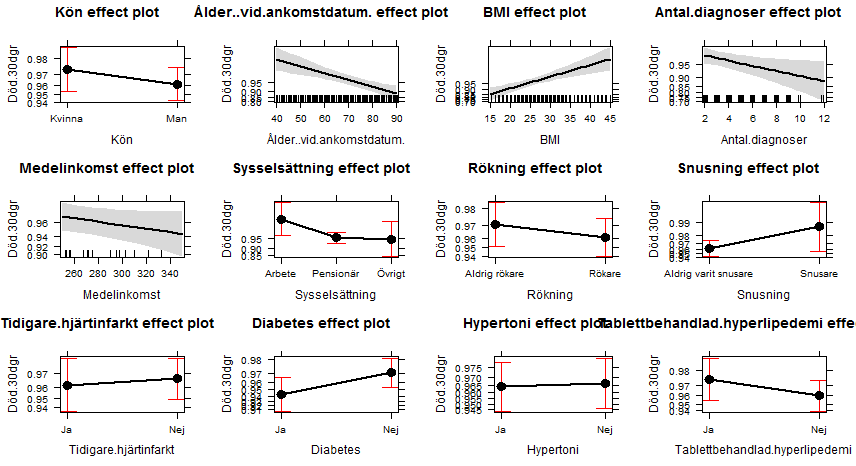
\includegraphics[width=0.8\textwidth]{effektmortalitet.png}
\end{minipage} 
\newpage
\section{Appendix 4 - Effektplot: Kostnad}
\noindent\begin{minipage}{\textwidth}

\centering
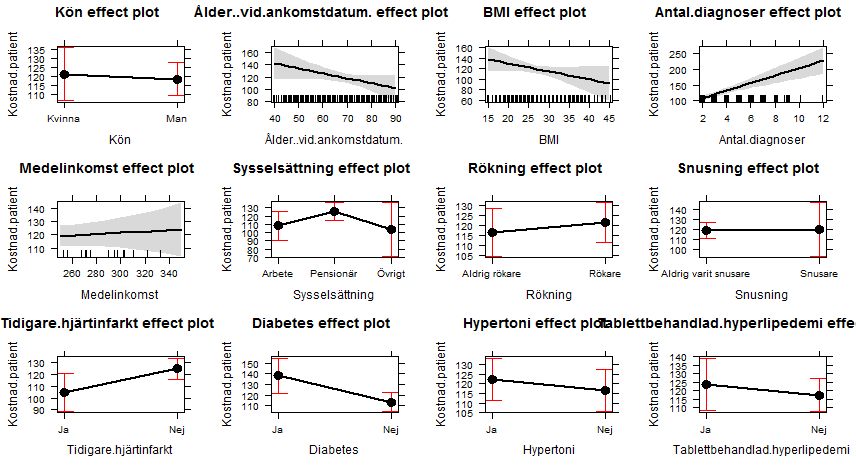
\includegraphics[width=0.8\textwidth]{effektkostnad.png}
\end{minipage} 
\newpage

%\section{Appendix 5 - R-Kod}
%\begin{lstlisting}[language=R]
%var kod
%\end{lstlisting}
%\newpage
\restoregeometry


%\bibliography{harvard}
\end{document}
